\documentclass[aspectratio=169]{beamer}
\usetheme{TUDelft}

% ====================================================================
% ANIMATION TOGGLE
% Set \animatedtrue for animated version with \cpause commands
% Set \animatedfalse for static version (all content visible at once)
% Use: pdflatex "\def\staticmode{1} \documentclass[aspectratio=169]{beamer}
\usetheme{TUDelft}

% ====================================================================
% ANIMATION TOGGLE
% Set \animatedtrue for animated version with \cpause commands
% Set \animatedfalse for static version (all content visible at once)
% Use: pdflatex "\def\staticmode{1} \documentclass[aspectratio=169]{beamer}
\usetheme{TUDelft}

% ====================================================================
% ANIMATION TOGGLE
% Set \animatedtrue for animated version with \cpause commands
% Set \animatedfalse for static version (all content visible at once)
% Use: pdflatex "\def\staticmode{1} \documentclass[aspectratio=169]{beamer}
\usetheme{TUDelft}

% ====================================================================
% ANIMATION TOGGLE
% Set \animatedtrue for animated version with \cpause commands
% Set \animatedfalse for static version (all content visible at once)
% Use: pdflatex "\def\staticmode{1} \input{01_intro_vector_space.tex}" for static version
% ====================================================================
\newif\ifanimated
\animatedtrue
\ifdefined\staticmode
  \animatedfalse
\fi

% Conditional pause command
\newcommand{\cpause}{\ifanimated\pause\fi}

% Packages
\usepackage{amsmath}
\usepackage{amssymb}
\usepackage{pifont} % For checkmarks and crosses if needed
\usepackage{amssymb}
\usepackage{algorithm}
\usepackage{algorithmic}
\usepackage{graphicx}
\usepackage{tikz}
\usepackage{booktabs}
\usepackage{listings}
\usepackage{xcolor}

% Python code styling
\lstset{
    language=Python,
    basicstyle=\ttfamily\footnotesize,
    keywordstyle=\color{blue},
    commentstyle=\color{gray},
    stringstyle=\color{red},
    showstringspaces=false,
    breaklines=true,
    frame=single,
    numbers=left,
    numberstyle=\tiny\color{gray}
}

% TikZ libraries
\usetikzlibrary{shapes,arrows,positioning,calc,patterns}

% Title information
\title[Introduction to IR]{Information Retrieval Introduction}
\subtitle{Lecture 1: Vector Space Model \& Boolean Retrieval}
\author{Avishek Anand}
\institute{Information Retrieval}
\date{\today}

\begin{document}

% Title slide
\begin{frame}
\titlepage
\end{frame}

% Course Overview
\begin{frame}{Course Overview}
\begin{enumerate}
    \item \textbf{Introduction to IR: Vector Space Model \& Boolean Retrieval} $\leftarrow$ Today
    \item Indexing: Sparse and Dense
    \item Query Understanding \& Expansion
    \item Evaluation of IR Systems
    \item Ranking: BM25, Language Models, and Beyond
    \item Embeddings \& Neural Ranking
    \item Dense Retrieval
    \item Learning to Rank
    \item Recommender Systems
    \item Retrieval Augmented Generation (RAG)
    \item LLMs as a Judge
\end{enumerate}
\cpause
\vspace{1em}
\textbf{Today's Goals:}
\begin{itemize}
    \item Understand what IR is and why it matters
    \item Learn the fundamental IR process
    \item Master Boolean retrieval and the vector space model
    % \item Build your first search engine
\end{itemize}
\end{frame}

\begin{frame}{Outline}
\tableofcontents
\end{frame}

% ====================================================================
% SECTION 1: WHAT IS INFORMATION RETRIEVAL?
% ====================================================================
\section{What is Information Retrieval?}
\begin{frame}
  \centering
  \LARGE \textbf{What is Information Retrieval?}
\end{frame}


\begin{frame}{What is Information Retrieval?}
\begin{block}{Definition}
Information Retrieval (IR) is finding material (usually documents) of an unstructured nature (usually text) that satisfies an information need from within large collections (usually stored on computers).
\end{block}
\cpause
\vspace{1em}

\begin{exampleblock}{The Essence of IR: Given an Information Need}
\begin{itemize}
    \item \textbf{Find relevant results} that satisfy the information need
    \item \textbf{By searching over a large collection} of items (billions of documents)
    \item \textbf{In reasonable time:}
    \begin{itemize}
        \item Web search: $< 1$ second
        \item AI/conversational systems: allow more time for generation
    \end{itemize}
    \item \textbf{Present results} in a manner that is easily consumable by humans
\end{itemize}
\end{exampleblock}
\end{frame}


\begin{frame}{IR vs. Database Systems}
\begin{table}
\centering
\begin{tabular}{lll}
\toprule
\textbf{Aspect} & \textbf{Database Systems} & \textbf{IR Systems} \\
\midrule
Data & Structured (tables, schemas) & Unstructured (text, documents) \\
Queries & Precise (SQL) & Vague (natural language) \\
Matching & Exact & Approximate/Ranked \\
Result & All matching records & Top-k relevant documents \\
Failure & No results or all results & Ranked list (best effort) \\
\midrule
Example & \texttt{SELECT * WHERE age>30} & ``climate change effects'' \\
\bottomrule
\end{tabular}
\end{table}

\vspace{1em}
\cpause

\begin{alertblock}{Key Difference}
Databases: \textit{``Give me all records matching X''} \\
IR: \textit{``Give me the most relevant documents about X''}
\end{alertblock}
\end{frame}

\begin{frame}[shrink]{IR vs. Natural Language Processing (NLP)}
\begin{block}{The Relationship}
IR and NLP are closely related but have different focal points:
\end{block}

\begin{columns}
\begin{column}{0.48\textwidth}
\textbf{NLP (Language Centric)}
\begin{itemize}
    \item Focus on language \textbf{understanding}, representation, and \textbf{generation}.
    \item Deep analysis of syntax, semantics, and pragmatics.
    \item Models like BERT, Llama, GPT.
\end{itemize}
\end{column}

\begin{column}{0.48\textwidth}
\textbf{IR (Scale \& Need Centric)}
\begin{itemize}
    \item Focus on \textbf{information seeking} at a massive scale.
    \item Uses NLP tech as a toolkit to model relevance.
    \item Priority: Speed, ranking, and satisfying user needs.
\end{itemize}
\end{column}
\end{columns}

\vspace{0.5em}

\begin{exampleblock}{Typical Tasks}
\begin{itemize}
    \item \textbf{NLP:} Named Entity Recognition, Dependency Parsing, Translation, Summarization.
    \item \textbf{IR:} Web Search, Recommendation Systems, Ad-hoc Retrieval, Question Answering.
\end{itemize}
\end{exampleblock}
\end{frame}


\begin{frame}[shrink=5]{Examples of Search Systems}
\begin{columns}
\begin{column}{0.48\textwidth}
\begin{center}
\textbf{Conversational AI Search}\\[0.5em]
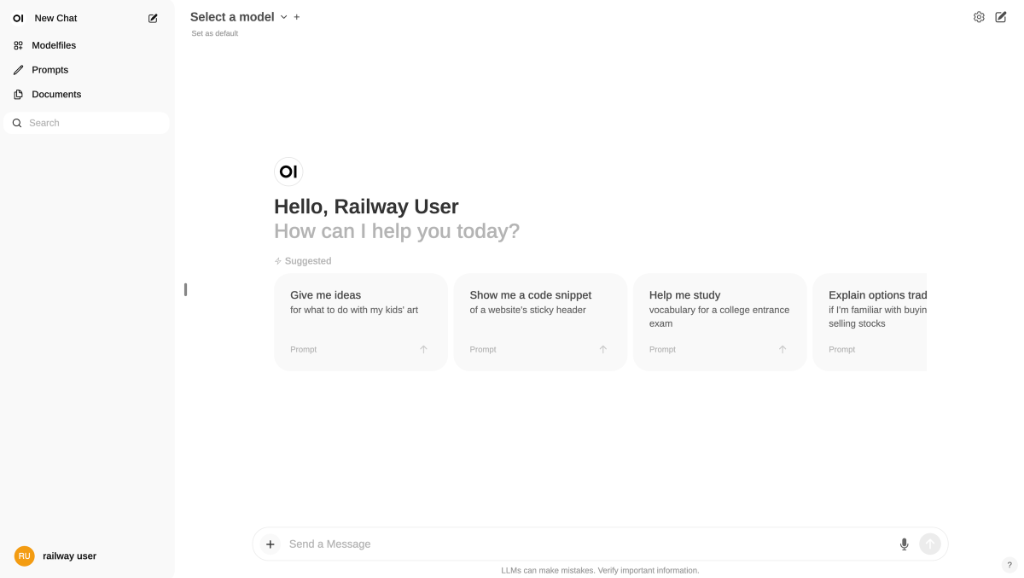
\includegraphics[width=\textwidth]{figures/search_chatgpt.png}\\
\small ChatGPT - AI-powered conversational search
\end{center}
\end{column}
\begin{column}{0.48\textwidth}
\begin{center}
\textbf{E-Commerce Search}\\[0.5em]
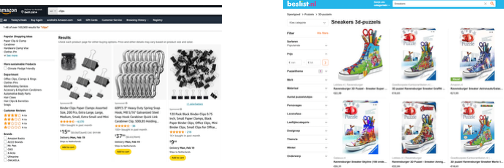
\includegraphics[width=\textwidth]{figures/search_amazon.png}\\
\small Amazon - Product search and recommendations
\end{center}
\end{column}
\end{columns}

\vspace{1em}
\begin{alertblock}{Common Thread}
All search systems share the same core challenge: finding relevant items from massive collections in real-time.
\end{alertblock}
\end{frame}

\begin{frame}{Real-World IR Applications}
\begin{columns}
\begin{column}{0.48\textwidth}
\textbf{Web Search}
\begin{itemize}
    \item Google, Bing, DuckDuckGo
    \item Billions of web pages
    \item Sub-second response time
\end{itemize}
\cpause
\vspace{1em}

\textbf{Enterprise Search}
\begin{itemize}
    \item Search company documents
    \item Email search
    \item Knowledge management
\end{itemize}
\cpause
\end{column}

\begin{column}{0.48\textwidth}
\textbf{E-commerce}
\begin{itemize}
    \item Amazon product search
    \item eBay, Etsy
    \item Recommendation systems
\end{itemize}
\cpause
\vspace{1em}

\textbf{Specialized Domains}
\begin{itemize}
    \item Legal document search (LexisNexis)
    \item Academic papers (Google Scholar)
    \item Medical records (PubMed)
    \item News archives
\end{itemize}
\end{column}
\end{columns}

\vspace{1em}

\begin{center}
\textbf{IR is everywhere you search for information!}
\end{center}
\end{frame}

% ====================================================================
% SECTION: CHALLENGES IN IR
% ====================================================================
\section{Challenges in IR}
\begin{frame}
  \centering
  \LARGE \textbf{Challenges in IR}
\end{frame}

\begin{frame}[shrink]{The Retrieval Challenge: Understanding Intent}
\begin{center}
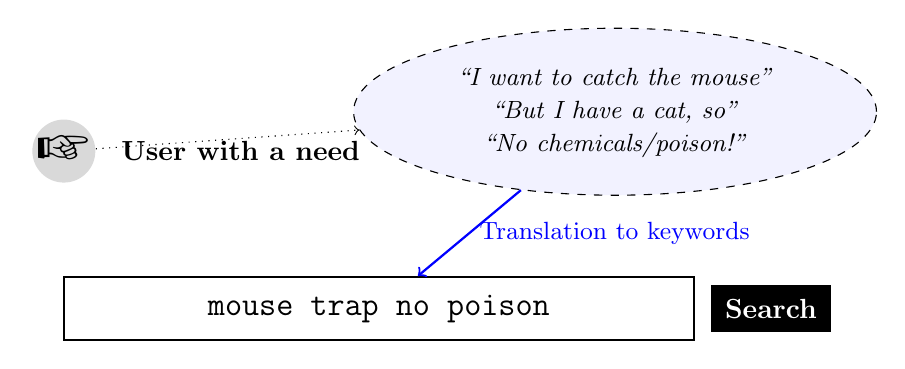
\begin{tikzpicture}[
    searchbox/.style={rectangle, draw, thick, minimum width=8cm, minimum height=0.8cm, font=\large},
    user/.style={circle, fill=gray!30, minimum size=0.8cm},
    icon/.style={font=\huge}
]
    % User Icon
    \node[user] (u) at (0,3) {};
    \node[icon] at (u) {\ding{43}}; % Hand/User representation
    \node[right=0.2cm of u] {\textbf{User with a need}};

    % Search Box
    \node[searchbox, fill=white] (box) at (4,1) {\texttt{mouse trap no poison}};
    \node[right=0.2cm of box, fill=black, text=white, inner sep=5pt] {\textbf{Search}};
    
    % Cloud / Intent
    \node[draw, ellipse, dashed, fill=blue!5, minimum width=4cm, minimum height=1.5cm] (intent) at (7,3.5) {
        \begin{tabular}{c}
            \small \textit{``I want to catch the mouse''} \\
            \small \textit{``But I have a cat, so''} \\
            \small \textit{``No chemicals/poison!''}
        \end{tabular}
    };
    \draw[->, dotted] (u) -- (intent);
    \draw[->, thick, blue] (intent) -- (box) node[midway, right] {\small Translation to keywords};
\end{tikzpicture}
\end{center}

\vspace{1em}
\begin{exampleblock}{The Semantic Gap}
\begin{itemize}
    \item \textbf{Syntactic match:} Docs containing ``mouse'', ``trap'', ``poison''.
    \item \textbf{User intent:} Docs describing \textit{humane} traps or \textit{mechanical} traps.
    \item \textbf{Danger:} Returning docs about ``how poison traps work'' (contains keywords!).
\end{itemize}
\end{exampleblock}
\end{frame}

\begin{frame}[shrink=5]{The Scale of Modern IR}
\begin{block}{Web Search Statistics (2024)}
\begin{itemize}
    \item \textbf{Google:} Processes 8.5+ billion searches per day
    \item \textbf{Index size:} 100+ trillion web pages indexed
    \item \textbf{Freshness:} New pages indexed within hours
    \item \textbf{Speed:} Results in $< 0.5$ seconds on average
\end{itemize}
\cpause
\end{block}
\vspace{1em}

\begin{exampleblock}{Challenges at Scale}
\begin{itemize}
    \item \textbf{Storage:} How to store 100 trillion documents?
    \item \textbf{Speed:} How to search in milliseconds?
    \item \textbf{Relevance:} How to rank billions of results?
    \item \textbf{Freshness:} How to keep index up-to-date?
    \item \textbf{Quality:} How to fight spam and misinformation?
\end{itemize}
\end{exampleblock}
\end{frame}

\begin{frame}[shrink=10]{The Information Retrieval Problem}
\begin{center}
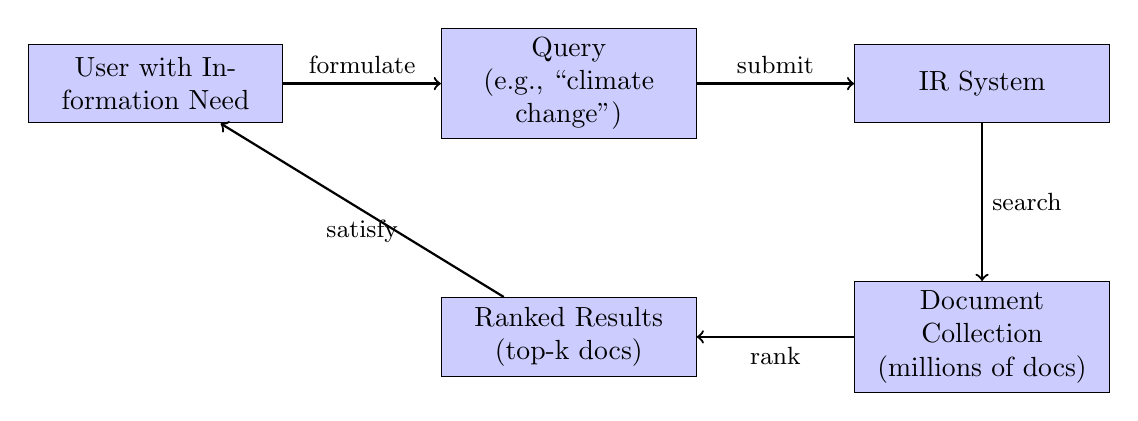
\begin{tikzpicture}[
    node distance=2cm,
    box/.style={rectangle, draw, fill=blue!20, text width=3cm, align=center, minimum height=1cm},
    arrow/.style={->, thick}
]
    \node[box] (user) {User with Information Need};
    \node[box, right=of user] (query) {Query \\ (e.g., ``climate change'')};
    \node[box, right=of query] (system) {IR System};
    \node[box, below=of system] (collection) {Document Collection \\ (millions of docs)};
    \node[box, left=of collection] (results) {Ranked Results \\ (top-k docs)};
    
    \draw[arrow] (user) -- (query) node[midway, above] {\small formulate};
    \draw[arrow] (query) -- (system) node[midway, above] {\small submit};
    \draw[arrow] (system) -- (collection) node[midway, right] {\small search};
    \draw[arrow] (collection) -- (results) node[midway, below] {\small rank};
    \draw[arrow] (results) -- (user) node[midway, below] {\small satisfy};
\end{tikzpicture}
\end{center}

\vspace{1em}
\cpause

\textbf{Core Questions:}
\begin{enumerate}
    \item How to represent documents and queries?
    \item How to match queries to documents efficiently?
    \item How to rank documents by relevance?
\end{enumerate}

\end{frame}

% ====================================================================
% ====================================================================
% SECTION 2: THE IR PROCESS (MOVED TO LECTURE 2)
% ====================================================================
\section{The Information Retrieval Process}
\begin{frame}{The Information Retrieval Process}
\begin{alertblock}{Forward Reference: Lecture 2}
\textbf{The fundamental IR process}, including pipeline architectures and preprocessing, is now covered in detail in \textbf{Lecture 2: Indexing}.
\end{alertblock}

\vspace{1em}
\begin{exampleblock}{Why the change?}
\begin{itemize}
    \item Better logical flow: Preprocessing is tightly coupled with building indexes.
    \item Focus for today: Understanding the models (Boolean and Vector Space).
\end{itemize}
\end{exampleblock}

\vspace{1em}
\begin{center}
\textit{Proceeding to Section 3: Boolean Retrieval...}
\end{center}
\end{frame}

% ====================================================================
% SECTION 3: BOOLEAN RETRIEVAL
% ====================================================================
\section{Boolean Retrieval}
\begin{frame}
  \centering
  \LARGE \textbf{Boolean Retrieval}
\end{frame}


\begin{frame}[shrink=5]{Boolean Retrieval Model}
\begin{block}{Definition}
Documents are retrieved if they satisfy a Boolean expression of query terms
\end{block}
\cpause
\vspace{1em}

\textbf{Boolean Operators:}
\begin{itemize}
    \item \textbf{AND:} Both terms must appear (intersection)
    \item \textbf{OR:} Either term must appear (union)
    \item \textbf{NOT:} Term must not appear (negation)
\end{itemize}
\cpause
\vspace{1em}

\begin{exampleblock}{Example Queries}
\begin{itemize}
    \item \texttt{climate AND change} → docs containing both ``climate'' and ``change''
    \item \texttt{cat OR dog} → docs containing ``cat'' or ``dog'' or both
    \item \texttt{java NOT coffee} → docs with ``java'' but not ``coffee''
    \item \texttt{(climate AND change) OR (global AND warming)}
\end{itemize}
% \cpause
\end{exampleblock}
% \cpause
\end{frame}

\begin{frame}{Boolean Retrieval with Sets}
\textbf{Documents as Sets of Terms}

\vspace{1em}

\begin{columns}
\begin{column}{0.48\textwidth}
\textbf{Document Collection:}
\begin{itemize}
    \item D1: \{cat, sat, mat\}
    \item D2: \{dog, sat, log\}
    \item D3: \{cat, dog, run\}
    \item D4: \{bird, fly, sky\}
\end{itemize}
\cpause
\end{column}

\begin{column}{0.48\textwidth}
\textbf{Inverted Index:}
\begin{itemize}
    \item cat: \{D1, D3\}
    \item dog: \{D2, D3\}
    \item sat: \{D1, D2\}
    \item run: \{D3\}
\end{itemize}
\cpause
\end{column}
\end{columns}

\vspace{1em}

\textbf{Query Processing:}
\begin{itemize}
    \item \texttt{cat AND dog}: \{D1, D3\} $\cap$ \{D2, D3\} = \{D3\}
    \item \texttt{cat OR dog}: \{D1, D3\} $\cup$ \{D2, D3\} = \{D1, D2, D3\}
    \item \texttt{cat NOT dog}: \{D1, D3\} - \{D2, D3\} = \{D1\}
\end{itemize}
% \cpause
\end{frame}

\begin{frame}[shrink=10]{Boolean Retrieval Example}
\textbf{Query:} \texttt{(cat AND mat) OR dog}

\vspace{1em}

\begin{center}
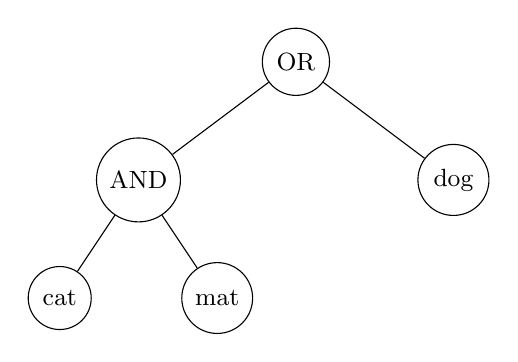
\begin{tikzpicture}[
    level distance=1.5cm,
    level 1/.style={sibling distance=4cm},
    level 2/.style={sibling distance=2cm},
    every node/.style={circle, draw, minimum size=0.8cm, font=\small}
]
    \node {OR}
        child {node {AND}
            child {node {cat}}
            child {node {mat}}
        }
        child {node {dog}};
\end{tikzpicture}
\end{center}

\vspace{1em}

\textbf{Execution:}
\begin{enumerate}
    \item \texttt{cat}: \{D1, D3\}
    \item \texttt{mat}: \{D1\}
    \item \texttt{cat AND mat}: \{D1, D3\} $\cap$ \{D1\} = \{D1\}
    \item \texttt{dog}: \{D2, D3\}
    \cpause
    \item \texttt{(cat AND mat) OR dog}: \{D1\} $\cup$ \{D2, D3\} = \{D1, D2, D3\}
\end{enumerate}
% \cpause
\end{frame}

\begin{frame}[shrink=10]{Advantages of Boolean Retrieval}
\begin{block}{\checkmark Advantages}
\begin{itemize}
    \item[\checkmark] \textbf{Precise control:} Users specify exactly what they want
    \item[\checkmark] \textbf{Transparent:} Clear why documents matched
    \item[\checkmark] \textbf{Efficient:} Fast set operations on posting lists
    \item[\checkmark] \textbf{Predictable:} Same query always returns same results
    \item[\checkmark] \textbf{Expressive:} Can construct complex queries
\end{itemize}
\cpause
\end{block}
% \cpause
\vspace{1em}

\begin{exampleblock}{Use Cases}
\begin{itemize}
    \item Legal document search (very precise requirements)
    \item Patent search (need exact specifications)
    \item Database-like queries on text
    \item Expert users who know what they want
\end{itemize}
% \cpause
\end{exampleblock}
% \cpause
\end{frame}

\begin{frame}{Limitations of Boolean Retrieval}
\begin{alertblock}{\ding{55} Critical Limitations}
\begin{enumerate}
    \item[\ding{55}] \textbf{No ranking}
    \begin{itemize}
        \item All matching documents equally relevant
        \item Can't distinguish ``very relevant'' from ``barely relevant''
    \end{itemize}
\cpause
    \item[\ding{55}] \textbf{All or nothing}
    \begin{itemize}
        \item \texttt{climate AND change AND effects}: No results if one term missing
        \item Too restrictive or too permissive
    \end{itemize}
\cpause
    \item[\ding{55}] \textbf{Hard to formulate queries}
    \begin{itemize}
        \item Most users don't know Boolean operators
        \item Hard to express fuzzy information needs
    \end{itemize}
\cpause
    \item[\ding{55}] \textbf{Result set size unpredictable}
    \begin{itemize}
        \item Could return 0 results or 10 million
        \item Users want ``top 10'', not ``all matching''
    \end{itemize}
% \cpause
\end{enumerate}
% \cpause
\end{alertblock}
% \cpause
\end{frame}

\begin{frame}{Boolean Retrieval: The Feast or Famine Problem}
\begin{columns}
\begin{column}{0.48\textwidth}
\textbf{Too Restrictive (Famine)}
\begin{itemize}
    \item Query: \texttt{machine AND learning AND neural AND networks}
    \item Result: 0 documents
    \item Problem: One term missing kills entire result
\end{itemize}
\cpause
\vspace{1em}

\textbf{Solution?}
\begin{itemize}
    \item User tries: \texttt{machine AND learning}
\end{itemize}
\cpause
\end{column}

\begin{column}{0.48\textwidth}
\textbf{Too Permissive (Feast)}
\begin{itemize}
    \item Query: \texttt{machine AND learning}
    \item Result: 1,000,000 documents
    \item Problem: Which 10 should I read?
\end{itemize}
\cpause
\vspace{1em}

\textbf{Need:}
\begin{itemize}
    \item Ranking by relevance
    \item Graceful degradation
    \item Better matching
\end{itemize}
% \cpause
\end{column}
\end{columns}

\vspace{1em}

\begin{center}
\textbf{This motivates the Vector Space Model!}
\end{center}
\end{frame}

% ====================================================================
% SECTION 4: VECTOR SPACE MODEL
% ====================================================================
\section{The Vector Space Model}
\begin{frame}
  \centering
  \LARGE \textbf{The Vector Space Model}
\end{frame}


\begin{frame}[shrink=10]{From Boolean to Vector Space}
\begin{block}{Key Insight}
Instead of documents being sets of terms (in/out), represent them as \textbf{vectors} with weights for each term
\end{block}
\cpause
\vspace{1em}

\begin{columns}
\begin{column}{0.48\textwidth}
\textbf{Boolean Model:}
\begin{itemize}
    \item D1: \{cat, dog\}
    \item D2: \{cat, mat\}
    \item Binary: term present or not
\end{itemize}
\cpause
\vspace{1em}

\textbf{Query:} \texttt{cat AND dog}
\begin{itemize}
    \item Result: \{D1\}
    \item D2 excluded (no ``dog'')
\end{itemize}
\cpause
\end{column}

\begin{column}{0.48\textwidth}
\textbf{Vector Space Model:}
\begin{itemize}
    \item D1: [cat: 0.5, dog: 0.5, mat: 0]
    \item D2: [cat: 0.7, dog: 0, mat: 0.3]
    \item Weighted: importance/frequency
\end{itemize}
\cpause
\vspace{1em}

\textbf{Query:} [cat: 0.5, dog: 0.5]
\begin{itemize}
    \item Similarity(D1, Q) = 0.5
    \item Similarity(D2, Q) = 0.35
    \item \textbf{Ranked:} D1, then D2
\end{itemize}
\cpause
\end{column}
\end{columns}

\vspace{1em}

\begin{exampleblock}{Advantage}
D2 still returned (has ``cat''), just ranked lower than D1
\end{exampleblock}
% \cpause
\end{frame}

\begin{frame}[shrink=10]{Vector Space Model: Geometric View}
\textbf{Documents and queries as vectors in term space}

\vspace{1em}

\begin{center}
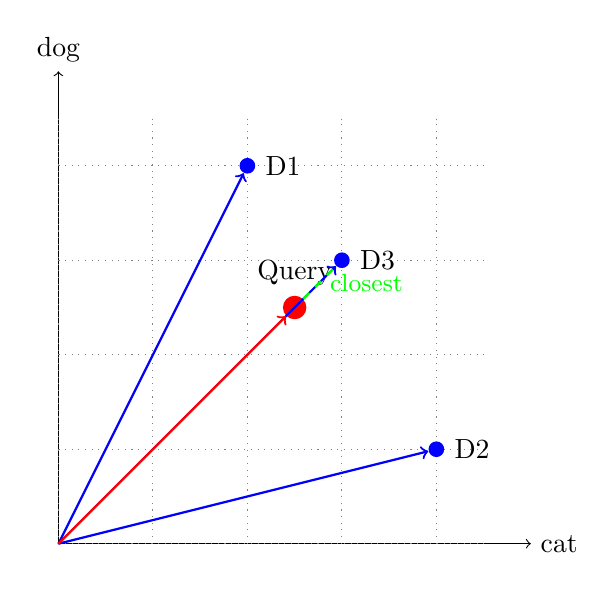
\begin{tikzpicture}[scale=1.2]
    % Axes
    \draw[->] (0,0) -- (5,0) node[right] {cat};
    \draw[->] (0,0) -- (0,5) node[above] {dog};
    
    % Grid
    \draw[gray, dotted] (0,0) grid (4.5,4.5);
    
    % Documents
    \node[circle, fill=blue, inner sep=2pt, label=right:D1] (d1) at (2,4) {};
    \node[circle, fill=blue, inner sep=2pt, label=right:D2] (d2) at (4,1) {};
    \node[circle, fill=blue, inner sep=2pt, label=right:D3] (d3) at (3,3) {};
    
    % Query
    \node[circle, fill=red, inner sep=3pt, label=above:Query] (q) at (2.5,2.5) {};
    
    % Vectors
    \draw[->, thick, blue] (0,0) -- (d1);
    \draw[->, thick, blue] (0,0) -- (d2);
    \draw[->, thick, blue] (0,0) -- (d3);
    \draw[->, thick, red] (0,0) -- (q);
    
    % Similarity illustration
    \draw[dashed, green, thick] (q) -- (d3) node[midway, right] {\small closest};
\end{tikzpicture}
\end{center}

\textbf{Similarity = Angle between vectors} \\
\small (Smaller angle = more similar)
\end{frame}

\begin{frame}[shrink=10]{Term Weighting in Vector Space Model}
\textbf{Question:} How to assign weights to terms?

\vspace{1em}

\begin{block}{Option 1: Binary Weights}
$$w_{t,d} = \begin{cases} 1 & \text{if term } t \text{ appears in doc } d \\ 0 & \text{otherwise} \end{cases}$$
\begin{itemize}
    \item Simple but ignores frequency
\end{itemize}
\cpause
\end{block}
\cpause
\begin{block}{Option 2: Term Frequency (TF)}
$$w_{t,d} = \text{count}(t, d)$$
\begin{itemize}
    \item Better: reflects importance
    \item Problem: Common words get high weight
\end{itemize}
\cpause
\end{block}
\cpause
\begin{alertblock}{Problem with Raw TF}
Document mentioning ``the'' 100 times doesn't make it about ``the''
\end{alertblock}
\cpause
\end{frame}

\begin{frame}[shrink=10]{TF-IDF Weighting}
\textbf{Idea:} Balance term frequency with term rarity

\vspace{1em}

\begin{block}{TF-IDF Formula}
$$w_{t,d} = \text{tf}(t,d) \times \text{idf}(t)$$

where:
\begin{itemize}
    \item $\text{tf}(t,d) = \text{count}(t,d)$ (term frequency in document)
    \item $\text{idf}(t) = \log\frac{N}{\text{df}(t)}$ (inverse document frequency)
    \item $N$ = total number of documents
    \item $\text{df}(t)$ = number of documents containing term $t$
\end{itemize}
\cpause
\end{block}
\cpause
\vspace{1em}

\textbf{Intuition:}
\begin{itemize}
    \item \textbf{High TF:} Term appears often in this document → important for this doc
    \item \textbf{High IDF:} Term is rare across collection → discriminative
    \item \textbf{High TF-IDF:} Important AND discriminative
\end{itemize}
% \cpause
\end{frame}

\begin{frame}[shrink=10]{TF-IDF Example}
\textbf{Collection:} 10,000 documents

\vspace{1em}

\begin{table}
\centering
\small
\begin{tabular}{lcccc}
\toprule
\textbf{Term} & \textbf{tf(t,d)} & \textbf{df(t)} & \textbf{idf(t)} & \textbf{tf-idf} \\
\midrule
neural & 5 & 100 & $\log(10000/100) = 2.0$ & 10.0 \\
network & 3 & 500 & $\log(10000/500) = 1.3$ & 3.9 \\
the & 50 & 9000 & $\log(10000/9000) = 0.05$ & 2.5 \\
\bottomrule
\end{tabular}
\end{table}

\vspace{1em}

\textbf{Observations:}
\begin{itemize}
    \item ``neural'' appears less than ``the'' (5 vs. 50) but gets higher weight (10.0 vs. 2.5)
    \item Rare, discriminative terms weighted higher
    \item Common words automatically downweighted
\end{itemize}
\cpause
\vspace{0.5em}

\begin{alertblock}{Note}
This is a simplified version; we'll cover refined TF-IDF and BM25 in Lecture 3
\end{alertblock}
\cpause
\end{frame}

\begin{frame}[shrink=10]{Document Vectors with TF-IDF}
\textbf{Example Collection:}
\begin{itemize}
    \item D1: ``cat cat dog''
    \item D2: ``cat mat''
    \item D3: ``dog bird bird''
\end{itemize}
\cpause
\vspace{1em}

\textbf{Vocabulary:} \{cat, dog, mat, bird\}

\vspace{1em}

\begin{table}
\centering
\small
\begin{tabular}{lcccc}
\toprule
\textbf{Doc} & \textbf{cat} & \textbf{dog} & \textbf{mat} & \textbf{bird} \\
\midrule
D1 & 2 × log(3/2) = 0.35 & 1 × log(3/2) = 0.18 & 0 & 0 \\
D2 & 1 × log(3/2) = 0.18 & 0 & 1 × log(3/1) = 0.48 & 0 \\
D3 & 0 & 1 × log(3/2) = 0.18 & 0 & 2 × log(3/1) = 0.95 \\
\bottomrule
\end{tabular}
\end{table}

\vspace{1em}

\textbf{Vector Representation:}
\begin{itemize}
    \item D1: [0.35, 0.18, 0, 0]
    \item D2: [0.18, 0, 0.48, 0]
    \item D3: [0, 0.18, 0, 0.95]
\end{itemize}
% \cpause
\end{frame}

\begin{frame}[shrink=10]{Cosine Similarity}
\textbf{How to measure similarity between vectors?}

\vspace{1em}

\begin{block}{Cosine Similarity Formula}
$$\text{sim}(\vec{q}, \vec{d}) = \frac{\vec{q} \cdot \vec{d}}{|\vec{q}| \times |\vec{d}|} = \frac{\sum_{t} q_t \times d_t}{\sqrt{\sum_{t} q_t^2} \times \sqrt{\sum_{t} d_t^2}}$$
\end{block}
\cpause
\vspace{1em}

\textbf{Properties:}
\begin{itemize}
    \item Range: [-1, 1] (or [0, 1] for positive weights)
    \item 1 = identical vectors (same direction)
    \item 0 = orthogonal (no common terms)
    \item -1 = opposite vectors (not relevant for IR)
\end{itemize}
\cpause
\vspace{1em}

\textbf{Why cosine instead of dot product?}
\begin{itemize}
    \item Cosine normalizes for document length
    \item Long documents don't automatically score higher
\end{itemize}
% \cpause
\end{frame}

\begin{frame}[shrink=10]{Cosine Similarity: Example Calculation}
\textbf{Query:} ``cat dog'' → $\vec{q} = [0.5, 0.5, 0, 0]$ \\
\textbf{Documents:}
\begin{itemize}
    \item D1: [0.35, 0.18, 0, 0]
    \item D2: [0.18, 0, 0.48, 0]
    \item D3: [0, 0.18, 0, 0.95]
\end{itemize}
\cpause
\vspace{1em}

\textbf{Similarity Calculations:}

\begin{align*}
\text{sim}(q, D1) &= \frac{(0.5 \times 0.35) + (0.5 \times 0.18)}{\sqrt{0.5^2 + 0.5^2} \times \sqrt{0.35^2 + 0.18^2}} \\
&= \frac{0.265}{0.707 \times 0.394} = 0.95 \\
\text{sim}(q, D2) &= \frac{0.5 \times 0.18}{0.707 \times 0.511} = 0.25 \\
\text{sim}(q, D3) &= \frac{0.5 \times 0.18}{0.707 \times 0.967} = 0.13
\end{align*}

\vspace{1em}

\textbf{Ranking:} D1 (0.95)  >  D2 (0.25)  >  D3 (0.13)
\end{frame}

\begin{frame}{VSM vs. Boolean Retrieval}
\begin{table}
\centering
\small
\begin{tabular}{lll}
\toprule
\textbf{Aspect} & \textbf{Boolean} & \textbf{Vector Space} \\
\midrule
Matching & Exact (in/out) & Partial (weighted) \\
Ranking & No & Yes (by similarity) \\
Result size & Unpredictable & Top-$k$ \\
Term weighting & Binary & TF-IDF \\
Query expression & Boolean operators & Term list \\
Robustness & Brittle & Graceful degradation \\
User friendliness & Expert users & General users \\
Relevance & All equal & Ranked by relevance \\
\bottomrule
\end{tabular}
\end{table}

\vspace{1em}

\begin{block}{Modern Usage}
\begin{itemize}
    \item \textbf{Boolean:} Still used in legal, patent search (precision critical)
    \item \textbf{Vector Space:} Foundation for web search, most IR systems
    \item \textbf{Hybrid:} Many systems combine both approaches
\end{itemize}
\cpause
\end{block}
\cpause
\end{frame}

\begin{frame}[shrink=5]{Advantages of Vector Space Model}
\begin{block}{\checkmark Key Advantages}
\begin{enumerate}
    \item \textbf{Ranking by relevance}
    \begin{itemize}
        \item Documents ordered by similarity to query
        \item Users get best results first
    \end{itemize}
\cpause
    \item \textbf{Partial matching}
    \begin{itemize}
        \item Documents matching some query terms still retrieved
        \item Graceful degradation (no feast/famine)
    \end{itemize}
\cpause
    \item \textbf{Term weighting}
    \begin{itemize}
        \item Important terms weighted higher (TF-IDF)
        \item Automatic handling of common words
    \end{itemize}
\cpause
    \item \textbf{Simple queries}
    \begin{itemize}
        \item Users just type terms (no Boolean operators)
        \item Natural for web search
    \end{itemize}
\cpause
    \item \textbf{Tunable}
    \begin{itemize}
        \item Can adjust weighting schemes
        \item Foundation for more advanced models (BM25, Lecture 3)
    \end{itemize}
\cpause
\end{enumerate}
\end{block}
\end{frame}

\begin{frame}[shrink=10]{Limitations of Vector Space Model}
\begin{alertblock}{\ding{55} Limitations}
\begin{enumerate}
    \item \textbf{Bag of words assumption}
    \begin{itemize}
        \item Word order ignored: ``dog bites man'' = ``man bites dog''
        \item No phrase matching
    \end{itemize}
\cpause
    \item \textbf{Term independence}
    \begin{itemize}
        \item Assumes terms are independent
        \item ``New York'' treated as ``New'' and ``York''
    \end{itemize}
\cpause
    \item \textbf{Synonymy}
    \begin{itemize}
        \item ``car'' and ``automobile'' treated as different
        \item Misses relevant documents with synonyms
    \end{itemize}
\cpause
    \item \textbf{Polysemy}
    \begin{itemize}
        \item ``bank'' (financial) vs. ``bank'' (river) undistinguished
        \item Can retrieve irrelevant documents
    \end{itemize}

\end{enumerate}

\end{alertblock}

\end{frame}


% ====================================================================
% SECTION 7: CONNECTIONS TO FUTURE LECTURES
% ====================================================================
\section{Questions}
\begin{frame}
  \centering
  \LARGE \textbf{Looking Ahead}
\end{frame}



\end{document}" for static version
% ====================================================================
\newif\ifanimated
\animatedtrue
\ifdefined\staticmode
  \animatedfalse
\fi

% Conditional pause command
\newcommand{\cpause}{\ifanimated\pause\fi}

% Packages
\usepackage{amsmath}
\usepackage{amssymb}
\usepackage{pifont} % For checkmarks and crosses if needed
\usepackage{amssymb}
\usepackage{algorithm}
\usepackage{algorithmic}
\usepackage{graphicx}
\usepackage{tikz}
\usepackage{booktabs}
\usepackage{listings}
\usepackage{xcolor}

% Python code styling
\lstset{
    language=Python,
    basicstyle=\ttfamily\footnotesize,
    keywordstyle=\color{blue},
    commentstyle=\color{gray},
    stringstyle=\color{red},
    showstringspaces=false,
    breaklines=true,
    frame=single,
    numbers=left,
    numberstyle=\tiny\color{gray}
}

% TikZ libraries
\usetikzlibrary{shapes,arrows,positioning,calc,patterns}

% Title information
\title[Introduction to IR]{Information Retrieval Introduction}
\subtitle{Lecture 1: Vector Space Model \& Boolean Retrieval}
\author{Avishek Anand}
\institute{Information Retrieval}
\date{\today}

\begin{document}

% Title slide
\begin{frame}
\titlepage
\end{frame}

% Course Overview
\begin{frame}{Course Overview}
\begin{enumerate}
    \item \textbf{Introduction to IR: Vector Space Model \& Boolean Retrieval} $\leftarrow$ Today
    \item Indexing: Sparse and Dense
    \item Query Understanding \& Expansion
    \item Evaluation of IR Systems
    \item Ranking: BM25, Language Models, and Beyond
    \item Embeddings \& Neural Ranking
    \item Dense Retrieval
    \item Learning to Rank
    \item Recommender Systems
    \item Retrieval Augmented Generation (RAG)
    \item LLMs as a Judge
\end{enumerate}
\cpause
\vspace{1em}
\textbf{Today's Goals:}
\begin{itemize}
    \item Understand what IR is and why it matters
    \item Learn the fundamental IR process
    \item Master Boolean retrieval and the vector space model
    % \item Build your first search engine
\end{itemize}
\end{frame}

\begin{frame}{Outline}
\tableofcontents
\end{frame}

% ====================================================================
% SECTION 1: WHAT IS INFORMATION RETRIEVAL?
% ====================================================================
\section{What is Information Retrieval?}
\begin{frame}
  \centering
  \LARGE \textbf{What is Information Retrieval?}
\end{frame}


\begin{frame}{What is Information Retrieval?}
\begin{block}{Definition}
Information Retrieval (IR) is finding material (usually documents) of an unstructured nature (usually text) that satisfies an information need from within large collections (usually stored on computers).
\end{block}
\cpause
\vspace{1em}

\begin{exampleblock}{The Essence of IR: Given an Information Need}
\begin{itemize}
    \item \textbf{Find relevant results} that satisfy the information need
    \item \textbf{By searching over a large collection} of items (billions of documents)
    \item \textbf{In reasonable time:}
    \begin{itemize}
        \item Web search: $< 1$ second
        \item AI/conversational systems: allow more time for generation
    \end{itemize}
    \item \textbf{Present results} in a manner that is easily consumable by humans
\end{itemize}
\end{exampleblock}
\end{frame}


\begin{frame}{IR vs. Database Systems}
\begin{table}
\centering
\begin{tabular}{lll}
\toprule
\textbf{Aspect} & \textbf{Database Systems} & \textbf{IR Systems} \\
\midrule
Data & Structured (tables, schemas) & Unstructured (text, documents) \\
Queries & Precise (SQL) & Vague (natural language) \\
Matching & Exact & Approximate/Ranked \\
Result & All matching records & Top-k relevant documents \\
Failure & No results or all results & Ranked list (best effort) \\
\midrule
Example & \texttt{SELECT * WHERE age>30} & ``climate change effects'' \\
\bottomrule
\end{tabular}
\end{table}

\vspace{1em}
\cpause

\begin{alertblock}{Key Difference}
Databases: \textit{``Give me all records matching X''} \\
IR: \textit{``Give me the most relevant documents about X''}
\end{alertblock}
\end{frame}

\begin{frame}[shrink]{IR vs. Natural Language Processing (NLP)}
\begin{block}{The Relationship}
IR and NLP are closely related but have different focal points:
\end{block}

\begin{columns}
\begin{column}{0.48\textwidth}
\textbf{NLP (Language Centric)}
\begin{itemize}
    \item Focus on language \textbf{understanding}, representation, and \textbf{generation}.
    \item Deep analysis of syntax, semantics, and pragmatics.
    \item Models like BERT, Llama, GPT.
\end{itemize}
\end{column}

\begin{column}{0.48\textwidth}
\textbf{IR (Scale \& Need Centric)}
\begin{itemize}
    \item Focus on \textbf{information seeking} at a massive scale.
    \item Uses NLP tech as a toolkit to model relevance.
    \item Priority: Speed, ranking, and satisfying user needs.
\end{itemize}
\end{column}
\end{columns}

\vspace{0.5em}

\begin{exampleblock}{Typical Tasks}
\begin{itemize}
    \item \textbf{NLP:} Named Entity Recognition, Dependency Parsing, Translation, Summarization.
    \item \textbf{IR:} Web Search, Recommendation Systems, Ad-hoc Retrieval, Question Answering.
\end{itemize}
\end{exampleblock}
\end{frame}


\begin{frame}[shrink=5]{Examples of Search Systems}
\begin{columns}
\begin{column}{0.48\textwidth}
\begin{center}
\textbf{Conversational AI Search}\\[0.5em]
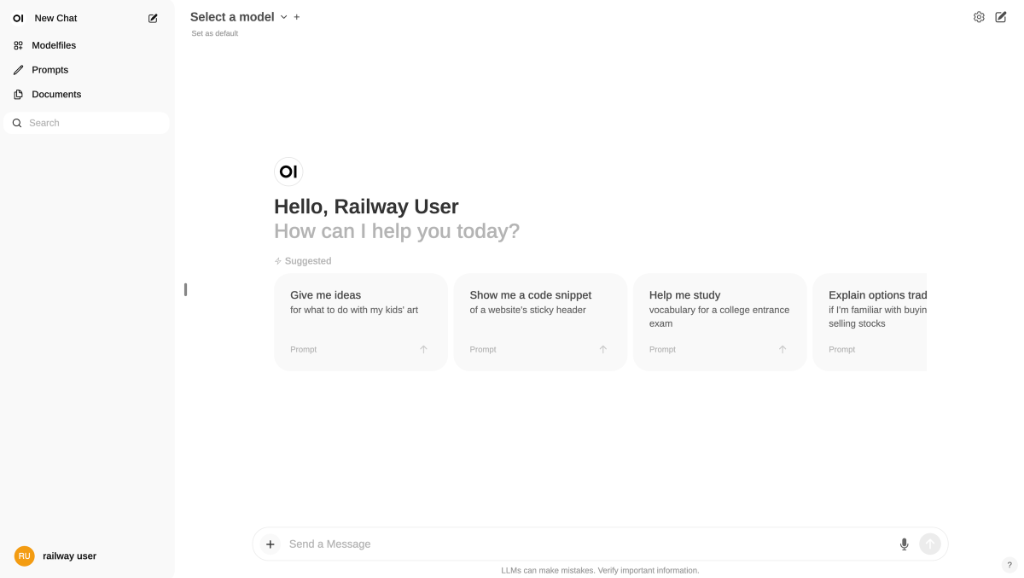
\includegraphics[width=\textwidth]{figures/search_chatgpt.png}\\
\small ChatGPT - AI-powered conversational search
\end{center}
\end{column}
\begin{column}{0.48\textwidth}
\begin{center}
\textbf{E-Commerce Search}\\[0.5em]
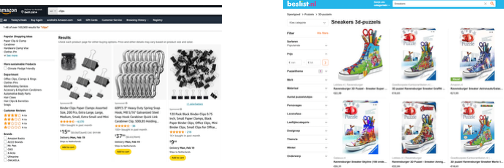
\includegraphics[width=\textwidth]{figures/search_amazon.png}\\
\small Amazon - Product search and recommendations
\end{center}
\end{column}
\end{columns}

\vspace{1em}
\begin{alertblock}{Common Thread}
All search systems share the same core challenge: finding relevant items from massive collections in real-time.
\end{alertblock}
\end{frame}

\begin{frame}{Real-World IR Applications}
\begin{columns}
\begin{column}{0.48\textwidth}
\textbf{Web Search}
\begin{itemize}
    \item Google, Bing, DuckDuckGo
    \item Billions of web pages
    \item Sub-second response time
\end{itemize}
\cpause
\vspace{1em}

\textbf{Enterprise Search}
\begin{itemize}
    \item Search company documents
    \item Email search
    \item Knowledge management
\end{itemize}
\cpause
\end{column}

\begin{column}{0.48\textwidth}
\textbf{E-commerce}
\begin{itemize}
    \item Amazon product search
    \item eBay, Etsy
    \item Recommendation systems
\end{itemize}
\cpause
\vspace{1em}

\textbf{Specialized Domains}
\begin{itemize}
    \item Legal document search (LexisNexis)
    \item Academic papers (Google Scholar)
    \item Medical records (PubMed)
    \item News archives
\end{itemize}
\end{column}
\end{columns}

\vspace{1em}

\begin{center}
\textbf{IR is everywhere you search for information!}
\end{center}
\end{frame}

% ====================================================================
% SECTION: CHALLENGES IN IR
% ====================================================================
\section{Challenges in IR}
\begin{frame}
  \centering
  \LARGE \textbf{Challenges in IR}
\end{frame}

\begin{frame}[shrink]{The Retrieval Challenge: Understanding Intent}
\begin{center}
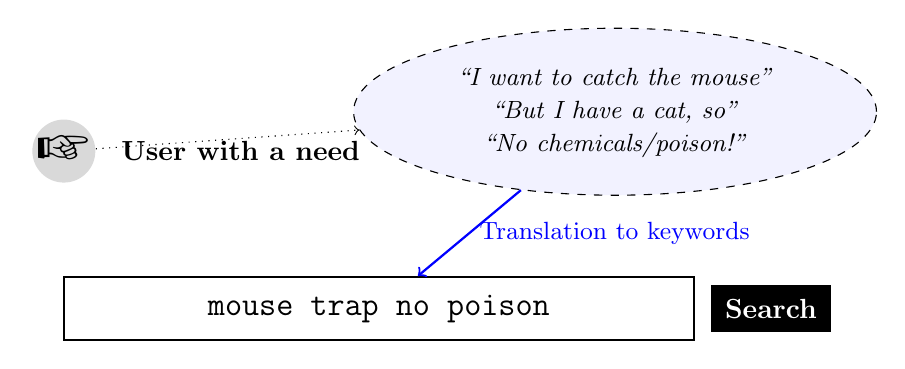
\begin{tikzpicture}[
    searchbox/.style={rectangle, draw, thick, minimum width=8cm, minimum height=0.8cm, font=\large},
    user/.style={circle, fill=gray!30, minimum size=0.8cm},
    icon/.style={font=\huge}
]
    % User Icon
    \node[user] (u) at (0,3) {};
    \node[icon] at (u) {\ding{43}}; % Hand/User representation
    \node[right=0.2cm of u] {\textbf{User with a need}};

    % Search Box
    \node[searchbox, fill=white] (box) at (4,1) {\texttt{mouse trap no poison}};
    \node[right=0.2cm of box, fill=black, text=white, inner sep=5pt] {\textbf{Search}};
    
    % Cloud / Intent
    \node[draw, ellipse, dashed, fill=blue!5, minimum width=4cm, minimum height=1.5cm] (intent) at (7,3.5) {
        \begin{tabular}{c}
            \small \textit{``I want to catch the mouse''} \\
            \small \textit{``But I have a cat, so''} \\
            \small \textit{``No chemicals/poison!''}
        \end{tabular}
    };
    \draw[->, dotted] (u) -- (intent);
    \draw[->, thick, blue] (intent) -- (box) node[midway, right] {\small Translation to keywords};
\end{tikzpicture}
\end{center}

\vspace{1em}
\begin{exampleblock}{The Semantic Gap}
\begin{itemize}
    \item \textbf{Syntactic match:} Docs containing ``mouse'', ``trap'', ``poison''.
    \item \textbf{User intent:} Docs describing \textit{humane} traps or \textit{mechanical} traps.
    \item \textbf{Danger:} Returning docs about ``how poison traps work'' (contains keywords!).
\end{itemize}
\end{exampleblock}
\end{frame}

\begin{frame}[shrink=5]{The Scale of Modern IR}
\begin{block}{Web Search Statistics (2024)}
\begin{itemize}
    \item \textbf{Google:} Processes 8.5+ billion searches per day
    \item \textbf{Index size:} 100+ trillion web pages indexed
    \item \textbf{Freshness:} New pages indexed within hours
    \item \textbf{Speed:} Results in $< 0.5$ seconds on average
\end{itemize}
\cpause
\end{block}
\vspace{1em}

\begin{exampleblock}{Challenges at Scale}
\begin{itemize}
    \item \textbf{Storage:} How to store 100 trillion documents?
    \item \textbf{Speed:} How to search in milliseconds?
    \item \textbf{Relevance:} How to rank billions of results?
    \item \textbf{Freshness:} How to keep index up-to-date?
    \item \textbf{Quality:} How to fight spam and misinformation?
\end{itemize}
\end{exampleblock}
\end{frame}

\begin{frame}[shrink=10]{The Information Retrieval Problem}
\begin{center}
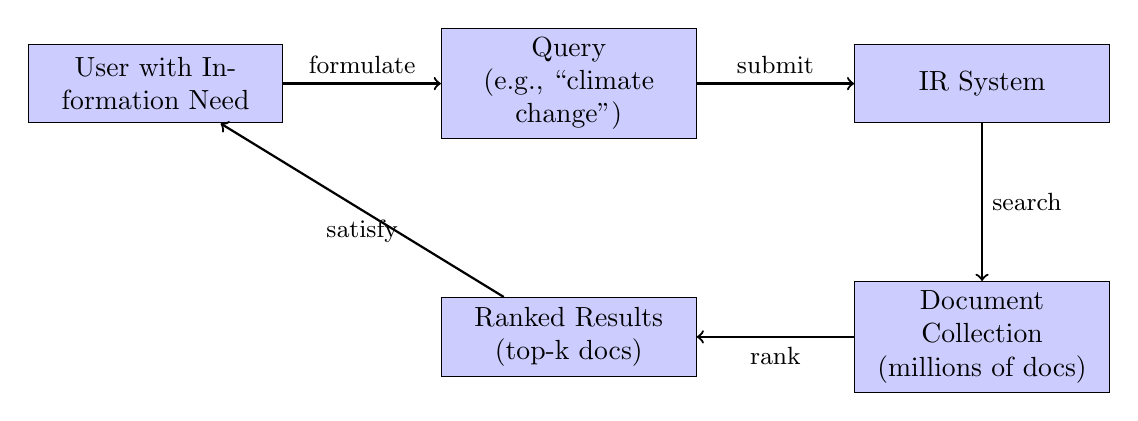
\begin{tikzpicture}[
    node distance=2cm,
    box/.style={rectangle, draw, fill=blue!20, text width=3cm, align=center, minimum height=1cm},
    arrow/.style={->, thick}
]
    \node[box] (user) {User with Information Need};
    \node[box, right=of user] (query) {Query \\ (e.g., ``climate change'')};
    \node[box, right=of query] (system) {IR System};
    \node[box, below=of system] (collection) {Document Collection \\ (millions of docs)};
    \node[box, left=of collection] (results) {Ranked Results \\ (top-k docs)};
    
    \draw[arrow] (user) -- (query) node[midway, above] {\small formulate};
    \draw[arrow] (query) -- (system) node[midway, above] {\small submit};
    \draw[arrow] (system) -- (collection) node[midway, right] {\small search};
    \draw[arrow] (collection) -- (results) node[midway, below] {\small rank};
    \draw[arrow] (results) -- (user) node[midway, below] {\small satisfy};
\end{tikzpicture}
\end{center}

\vspace{1em}
\cpause

\textbf{Core Questions:}
\begin{enumerate}
    \item How to represent documents and queries?
    \item How to match queries to documents efficiently?
    \item How to rank documents by relevance?
\end{enumerate}

\end{frame}

% ====================================================================
% ====================================================================
% SECTION 2: THE IR PROCESS (MOVED TO LECTURE 2)
% ====================================================================
\section{The Information Retrieval Process}
\begin{frame}{The Information Retrieval Process}
\begin{alertblock}{Forward Reference: Lecture 2}
\textbf{The fundamental IR process}, including pipeline architectures and preprocessing, is now covered in detail in \textbf{Lecture 2: Indexing}.
\end{alertblock}

\vspace{1em}
\begin{exampleblock}{Why the change?}
\begin{itemize}
    \item Better logical flow: Preprocessing is tightly coupled with building indexes.
    \item Focus for today: Understanding the models (Boolean and Vector Space).
\end{itemize}
\end{exampleblock}

\vspace{1em}
\begin{center}
\textit{Proceeding to Section 3: Boolean Retrieval...}
\end{center}
\end{frame}

% ====================================================================
% SECTION 3: BOOLEAN RETRIEVAL
% ====================================================================
\section{Boolean Retrieval}
\begin{frame}
  \centering
  \LARGE \textbf{Boolean Retrieval}
\end{frame}


\begin{frame}[shrink=5]{Boolean Retrieval Model}
\begin{block}{Definition}
Documents are retrieved if they satisfy a Boolean expression of query terms
\end{block}
\cpause
\vspace{1em}

\textbf{Boolean Operators:}
\begin{itemize}
    \item \textbf{AND:} Both terms must appear (intersection)
    \item \textbf{OR:} Either term must appear (union)
    \item \textbf{NOT:} Term must not appear (negation)
\end{itemize}
\cpause
\vspace{1em}

\begin{exampleblock}{Example Queries}
\begin{itemize}
    \item \texttt{climate AND change} → docs containing both ``climate'' and ``change''
    \item \texttt{cat OR dog} → docs containing ``cat'' or ``dog'' or both
    \item \texttt{java NOT coffee} → docs with ``java'' but not ``coffee''
    \item \texttt{(climate AND change) OR (global AND warming)}
\end{itemize}
% \cpause
\end{exampleblock}
% \cpause
\end{frame}

\begin{frame}{Boolean Retrieval with Sets}
\textbf{Documents as Sets of Terms}

\vspace{1em}

\begin{columns}
\begin{column}{0.48\textwidth}
\textbf{Document Collection:}
\begin{itemize}
    \item D1: \{cat, sat, mat\}
    \item D2: \{dog, sat, log\}
    \item D3: \{cat, dog, run\}
    \item D4: \{bird, fly, sky\}
\end{itemize}
\cpause
\end{column}

\begin{column}{0.48\textwidth}
\textbf{Inverted Index:}
\begin{itemize}
    \item cat: \{D1, D3\}
    \item dog: \{D2, D3\}
    \item sat: \{D1, D2\}
    \item run: \{D3\}
\end{itemize}
\cpause
\end{column}
\end{columns}

\vspace{1em}

\textbf{Query Processing:}
\begin{itemize}
    \item \texttt{cat AND dog}: \{D1, D3\} $\cap$ \{D2, D3\} = \{D3\}
    \item \texttt{cat OR dog}: \{D1, D3\} $\cup$ \{D2, D3\} = \{D1, D2, D3\}
    \item \texttt{cat NOT dog}: \{D1, D3\} - \{D2, D3\} = \{D1\}
\end{itemize}
% \cpause
\end{frame}

\begin{frame}[shrink=10]{Boolean Retrieval Example}
\textbf{Query:} \texttt{(cat AND mat) OR dog}

\vspace{1em}

\begin{center}
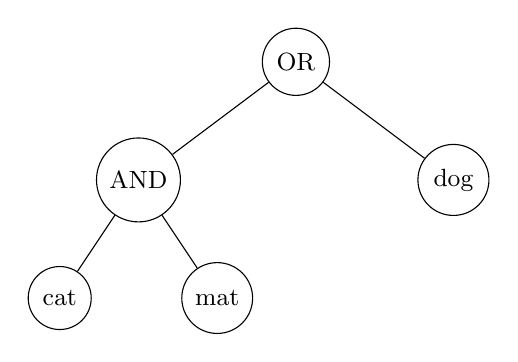
\begin{tikzpicture}[
    level distance=1.5cm,
    level 1/.style={sibling distance=4cm},
    level 2/.style={sibling distance=2cm},
    every node/.style={circle, draw, minimum size=0.8cm, font=\small}
]
    \node {OR}
        child {node {AND}
            child {node {cat}}
            child {node {mat}}
        }
        child {node {dog}};
\end{tikzpicture}
\end{center}

\vspace{1em}

\textbf{Execution:}
\begin{enumerate}
    \item \texttt{cat}: \{D1, D3\}
    \item \texttt{mat}: \{D1\}
    \item \texttt{cat AND mat}: \{D1, D3\} $\cap$ \{D1\} = \{D1\}
    \item \texttt{dog}: \{D2, D3\}
    \cpause
    \item \texttt{(cat AND mat) OR dog}: \{D1\} $\cup$ \{D2, D3\} = \{D1, D2, D3\}
\end{enumerate}
% \cpause
\end{frame}

\begin{frame}[shrink=10]{Advantages of Boolean Retrieval}
\begin{block}{\checkmark Advantages}
\begin{itemize}
    \item[\checkmark] \textbf{Precise control:} Users specify exactly what they want
    \item[\checkmark] \textbf{Transparent:} Clear why documents matched
    \item[\checkmark] \textbf{Efficient:} Fast set operations on posting lists
    \item[\checkmark] \textbf{Predictable:} Same query always returns same results
    \item[\checkmark] \textbf{Expressive:} Can construct complex queries
\end{itemize}
\cpause
\end{block}
% \cpause
\vspace{1em}

\begin{exampleblock}{Use Cases}
\begin{itemize}
    \item Legal document search (very precise requirements)
    \item Patent search (need exact specifications)
    \item Database-like queries on text
    \item Expert users who know what they want
\end{itemize}
% \cpause
\end{exampleblock}
% \cpause
\end{frame}

\begin{frame}{Limitations of Boolean Retrieval}
\begin{alertblock}{\ding{55} Critical Limitations}
\begin{enumerate}
    \item[\ding{55}] \textbf{No ranking}
    \begin{itemize}
        \item All matching documents equally relevant
        \item Can't distinguish ``very relevant'' from ``barely relevant''
    \end{itemize}
\cpause
    \item[\ding{55}] \textbf{All or nothing}
    \begin{itemize}
        \item \texttt{climate AND change AND effects}: No results if one term missing
        \item Too restrictive or too permissive
    \end{itemize}
\cpause
    \item[\ding{55}] \textbf{Hard to formulate queries}
    \begin{itemize}
        \item Most users don't know Boolean operators
        \item Hard to express fuzzy information needs
    \end{itemize}
\cpause
    \item[\ding{55}] \textbf{Result set size unpredictable}
    \begin{itemize}
        \item Could return 0 results or 10 million
        \item Users want ``top 10'', not ``all matching''
    \end{itemize}
% \cpause
\end{enumerate}
% \cpause
\end{alertblock}
% \cpause
\end{frame}

\begin{frame}{Boolean Retrieval: The Feast or Famine Problem}
\begin{columns}
\begin{column}{0.48\textwidth}
\textbf{Too Restrictive (Famine)}
\begin{itemize}
    \item Query: \texttt{machine AND learning AND neural AND networks}
    \item Result: 0 documents
    \item Problem: One term missing kills entire result
\end{itemize}
\cpause
\vspace{1em}

\textbf{Solution?}
\begin{itemize}
    \item User tries: \texttt{machine AND learning}
\end{itemize}
\cpause
\end{column}

\begin{column}{0.48\textwidth}
\textbf{Too Permissive (Feast)}
\begin{itemize}
    \item Query: \texttt{machine AND learning}
    \item Result: 1,000,000 documents
    \item Problem: Which 10 should I read?
\end{itemize}
\cpause
\vspace{1em}

\textbf{Need:}
\begin{itemize}
    \item Ranking by relevance
    \item Graceful degradation
    \item Better matching
\end{itemize}
% \cpause
\end{column}
\end{columns}

\vspace{1em}

\begin{center}
\textbf{This motivates the Vector Space Model!}
\end{center}
\end{frame}

% ====================================================================
% SECTION 4: VECTOR SPACE MODEL
% ====================================================================
\section{The Vector Space Model}
\begin{frame}
  \centering
  \LARGE \textbf{The Vector Space Model}
\end{frame}


\begin{frame}[shrink=10]{From Boolean to Vector Space}
\begin{block}{Key Insight}
Instead of documents being sets of terms (in/out), represent them as \textbf{vectors} with weights for each term
\end{block}
\cpause
\vspace{1em}

\begin{columns}
\begin{column}{0.48\textwidth}
\textbf{Boolean Model:}
\begin{itemize}
    \item D1: \{cat, dog\}
    \item D2: \{cat, mat\}
    \item Binary: term present or not
\end{itemize}
\cpause
\vspace{1em}

\textbf{Query:} \texttt{cat AND dog}
\begin{itemize}
    \item Result: \{D1\}
    \item D2 excluded (no ``dog'')
\end{itemize}
\cpause
\end{column}

\begin{column}{0.48\textwidth}
\textbf{Vector Space Model:}
\begin{itemize}
    \item D1: [cat: 0.5, dog: 0.5, mat: 0]
    \item D2: [cat: 0.7, dog: 0, mat: 0.3]
    \item Weighted: importance/frequency
\end{itemize}
\cpause
\vspace{1em}

\textbf{Query:} [cat: 0.5, dog: 0.5]
\begin{itemize}
    \item Similarity(D1, Q) = 0.5
    \item Similarity(D2, Q) = 0.35
    \item \textbf{Ranked:} D1, then D2
\end{itemize}
\cpause
\end{column}
\end{columns}

\vspace{1em}

\begin{exampleblock}{Advantage}
D2 still returned (has ``cat''), just ranked lower than D1
\end{exampleblock}
% \cpause
\end{frame}

\begin{frame}[shrink=10]{Vector Space Model: Geometric View}
\textbf{Documents and queries as vectors in term space}

\vspace{1em}

\begin{center}
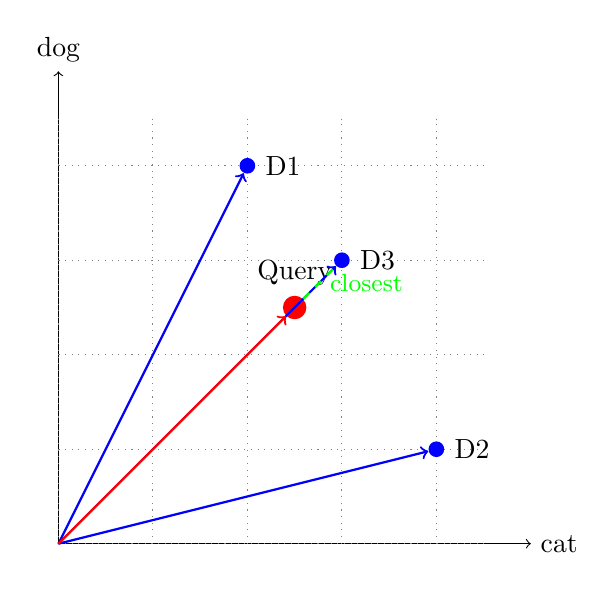
\begin{tikzpicture}[scale=1.2]
    % Axes
    \draw[->] (0,0) -- (5,0) node[right] {cat};
    \draw[->] (0,0) -- (0,5) node[above] {dog};
    
    % Grid
    \draw[gray, dotted] (0,0) grid (4.5,4.5);
    
    % Documents
    \node[circle, fill=blue, inner sep=2pt, label=right:D1] (d1) at (2,4) {};
    \node[circle, fill=blue, inner sep=2pt, label=right:D2] (d2) at (4,1) {};
    \node[circle, fill=blue, inner sep=2pt, label=right:D3] (d3) at (3,3) {};
    
    % Query
    \node[circle, fill=red, inner sep=3pt, label=above:Query] (q) at (2.5,2.5) {};
    
    % Vectors
    \draw[->, thick, blue] (0,0) -- (d1);
    \draw[->, thick, blue] (0,0) -- (d2);
    \draw[->, thick, blue] (0,0) -- (d3);
    \draw[->, thick, red] (0,0) -- (q);
    
    % Similarity illustration
    \draw[dashed, green, thick] (q) -- (d3) node[midway, right] {\small closest};
\end{tikzpicture}
\end{center}

\textbf{Similarity = Angle between vectors} \\
\small (Smaller angle = more similar)
\end{frame}

\begin{frame}[shrink=10]{Term Weighting in Vector Space Model}
\textbf{Question:} How to assign weights to terms?

\vspace{1em}

\begin{block}{Option 1: Binary Weights}
$$w_{t,d} = \begin{cases} 1 & \text{if term } t \text{ appears in doc } d \\ 0 & \text{otherwise} \end{cases}$$
\begin{itemize}
    \item Simple but ignores frequency
\end{itemize}
\cpause
\end{block}
\cpause
\begin{block}{Option 2: Term Frequency (TF)}
$$w_{t,d} = \text{count}(t, d)$$
\begin{itemize}
    \item Better: reflects importance
    \item Problem: Common words get high weight
\end{itemize}
\cpause
\end{block}
\cpause
\begin{alertblock}{Problem with Raw TF}
Document mentioning ``the'' 100 times doesn't make it about ``the''
\end{alertblock}
\cpause
\end{frame}

\begin{frame}[shrink=10]{TF-IDF Weighting}
\textbf{Idea:} Balance term frequency with term rarity

\vspace{1em}

\begin{block}{TF-IDF Formula}
$$w_{t,d} = \text{tf}(t,d) \times \text{idf}(t)$$

where:
\begin{itemize}
    \item $\text{tf}(t,d) = \text{count}(t,d)$ (term frequency in document)
    \item $\text{idf}(t) = \log\frac{N}{\text{df}(t)}$ (inverse document frequency)
    \item $N$ = total number of documents
    \item $\text{df}(t)$ = number of documents containing term $t$
\end{itemize}
\cpause
\end{block}
\cpause
\vspace{1em}

\textbf{Intuition:}
\begin{itemize}
    \item \textbf{High TF:} Term appears often in this document → important for this doc
    \item \textbf{High IDF:} Term is rare across collection → discriminative
    \item \textbf{High TF-IDF:} Important AND discriminative
\end{itemize}
% \cpause
\end{frame}

\begin{frame}[shrink=10]{TF-IDF Example}
\textbf{Collection:} 10,000 documents

\vspace{1em}

\begin{table}
\centering
\small
\begin{tabular}{lcccc}
\toprule
\textbf{Term} & \textbf{tf(t,d)} & \textbf{df(t)} & \textbf{idf(t)} & \textbf{tf-idf} \\
\midrule
neural & 5 & 100 & $\log(10000/100) = 2.0$ & 10.0 \\
network & 3 & 500 & $\log(10000/500) = 1.3$ & 3.9 \\
the & 50 & 9000 & $\log(10000/9000) = 0.05$ & 2.5 \\
\bottomrule
\end{tabular}
\end{table}

\vspace{1em}

\textbf{Observations:}
\begin{itemize}
    \item ``neural'' appears less than ``the'' (5 vs. 50) but gets higher weight (10.0 vs. 2.5)
    \item Rare, discriminative terms weighted higher
    \item Common words automatically downweighted
\end{itemize}
\cpause
\vspace{0.5em}

\begin{alertblock}{Note}
This is a simplified version; we'll cover refined TF-IDF and BM25 in Lecture 3
\end{alertblock}
\cpause
\end{frame}

\begin{frame}[shrink=10]{Document Vectors with TF-IDF}
\textbf{Example Collection:}
\begin{itemize}
    \item D1: ``cat cat dog''
    \item D2: ``cat mat''
    \item D3: ``dog bird bird''
\end{itemize}
\cpause
\vspace{1em}

\textbf{Vocabulary:} \{cat, dog, mat, bird\}

\vspace{1em}

\begin{table}
\centering
\small
\begin{tabular}{lcccc}
\toprule
\textbf{Doc} & \textbf{cat} & \textbf{dog} & \textbf{mat} & \textbf{bird} \\
\midrule
D1 & 2 × log(3/2) = 0.35 & 1 × log(3/2) = 0.18 & 0 & 0 \\
D2 & 1 × log(3/2) = 0.18 & 0 & 1 × log(3/1) = 0.48 & 0 \\
D3 & 0 & 1 × log(3/2) = 0.18 & 0 & 2 × log(3/1) = 0.95 \\
\bottomrule
\end{tabular}
\end{table}

\vspace{1em}

\textbf{Vector Representation:}
\begin{itemize}
    \item D1: [0.35, 0.18, 0, 0]
    \item D2: [0.18, 0, 0.48, 0]
    \item D3: [0, 0.18, 0, 0.95]
\end{itemize}
% \cpause
\end{frame}

\begin{frame}[shrink=10]{Cosine Similarity}
\textbf{How to measure similarity between vectors?}

\vspace{1em}

\begin{block}{Cosine Similarity Formula}
$$\text{sim}(\vec{q}, \vec{d}) = \frac{\vec{q} \cdot \vec{d}}{|\vec{q}| \times |\vec{d}|} = \frac{\sum_{t} q_t \times d_t}{\sqrt{\sum_{t} q_t^2} \times \sqrt{\sum_{t} d_t^2}}$$
\end{block}
\cpause
\vspace{1em}

\textbf{Properties:}
\begin{itemize}
    \item Range: [-1, 1] (or [0, 1] for positive weights)
    \item 1 = identical vectors (same direction)
    \item 0 = orthogonal (no common terms)
    \item -1 = opposite vectors (not relevant for IR)
\end{itemize}
\cpause
\vspace{1em}

\textbf{Why cosine instead of dot product?}
\begin{itemize}
    \item Cosine normalizes for document length
    \item Long documents don't automatically score higher
\end{itemize}
% \cpause
\end{frame}

\begin{frame}[shrink=10]{Cosine Similarity: Example Calculation}
\textbf{Query:} ``cat dog'' → $\vec{q} = [0.5, 0.5, 0, 0]$ \\
\textbf{Documents:}
\begin{itemize}
    \item D1: [0.35, 0.18, 0, 0]
    \item D2: [0.18, 0, 0.48, 0]
    \item D3: [0, 0.18, 0, 0.95]
\end{itemize}
\cpause
\vspace{1em}

\textbf{Similarity Calculations:}

\begin{align*}
\text{sim}(q, D1) &= \frac{(0.5 \times 0.35) + (0.5 \times 0.18)}{\sqrt{0.5^2 + 0.5^2} \times \sqrt{0.35^2 + 0.18^2}} \\
&= \frac{0.265}{0.707 \times 0.394} = 0.95 \\
\text{sim}(q, D2) &= \frac{0.5 \times 0.18}{0.707 \times 0.511} = 0.25 \\
\text{sim}(q, D3) &= \frac{0.5 \times 0.18}{0.707 \times 0.967} = 0.13
\end{align*}

\vspace{1em}

\textbf{Ranking:} D1 (0.95)  >  D2 (0.25)  >  D3 (0.13)
\end{frame}

\begin{frame}{VSM vs. Boolean Retrieval}
\begin{table}
\centering
\small
\begin{tabular}{lll}
\toprule
\textbf{Aspect} & \textbf{Boolean} & \textbf{Vector Space} \\
\midrule
Matching & Exact (in/out) & Partial (weighted) \\
Ranking & No & Yes (by similarity) \\
Result size & Unpredictable & Top-$k$ \\
Term weighting & Binary & TF-IDF \\
Query expression & Boolean operators & Term list \\
Robustness & Brittle & Graceful degradation \\
User friendliness & Expert users & General users \\
Relevance & All equal & Ranked by relevance \\
\bottomrule
\end{tabular}
\end{table}

\vspace{1em}

\begin{block}{Modern Usage}
\begin{itemize}
    \item \textbf{Boolean:} Still used in legal, patent search (precision critical)
    \item \textbf{Vector Space:} Foundation for web search, most IR systems
    \item \textbf{Hybrid:} Many systems combine both approaches
\end{itemize}
\cpause
\end{block}
\cpause
\end{frame}

\begin{frame}[shrink=5]{Advantages of Vector Space Model}
\begin{block}{\checkmark Key Advantages}
\begin{enumerate}
    \item \textbf{Ranking by relevance}
    \begin{itemize}
        \item Documents ordered by similarity to query
        \item Users get best results first
    \end{itemize}
\cpause
    \item \textbf{Partial matching}
    \begin{itemize}
        \item Documents matching some query terms still retrieved
        \item Graceful degradation (no feast/famine)
    \end{itemize}
\cpause
    \item \textbf{Term weighting}
    \begin{itemize}
        \item Important terms weighted higher (TF-IDF)
        \item Automatic handling of common words
    \end{itemize}
\cpause
    \item \textbf{Simple queries}
    \begin{itemize}
        \item Users just type terms (no Boolean operators)
        \item Natural for web search
    \end{itemize}
\cpause
    \item \textbf{Tunable}
    \begin{itemize}
        \item Can adjust weighting schemes
        \item Foundation for more advanced models (BM25, Lecture 3)
    \end{itemize}
\cpause
\end{enumerate}
\end{block}
\end{frame}

\begin{frame}[shrink=10]{Limitations of Vector Space Model}
\begin{alertblock}{\ding{55} Limitations}
\begin{enumerate}
    \item \textbf{Bag of words assumption}
    \begin{itemize}
        \item Word order ignored: ``dog bites man'' = ``man bites dog''
        \item No phrase matching
    \end{itemize}
\cpause
    \item \textbf{Term independence}
    \begin{itemize}
        \item Assumes terms are independent
        \item ``New York'' treated as ``New'' and ``York''
    \end{itemize}
\cpause
    \item \textbf{Synonymy}
    \begin{itemize}
        \item ``car'' and ``automobile'' treated as different
        \item Misses relevant documents with synonyms
    \end{itemize}
\cpause
    \item \textbf{Polysemy}
    \begin{itemize}
        \item ``bank'' (financial) vs. ``bank'' (river) undistinguished
        \item Can retrieve irrelevant documents
    \end{itemize}

\end{enumerate}

\end{alertblock}

\end{frame}


% ====================================================================
% SECTION 7: CONNECTIONS TO FUTURE LECTURES
% ====================================================================
\section{Questions}
\begin{frame}
  \centering
  \LARGE \textbf{Looking Ahead}
\end{frame}



\end{document}" for static version
% ====================================================================
\newif\ifanimated
\animatedtrue
\ifdefined\staticmode
  \animatedfalse
\fi

% Conditional pause command
\newcommand{\cpause}{\ifanimated\pause\fi}

% Packages
\usepackage{amsmath}
\usepackage{amssymb}
\usepackage{pifont} % For checkmarks and crosses if needed
\usepackage{amssymb}
\usepackage{algorithm}
\usepackage{algorithmic}
\usepackage{graphicx}
\usepackage{tikz}
\usepackage{booktabs}
\usepackage{listings}
\usepackage{xcolor}

% Python code styling
\lstset{
    language=Python,
    basicstyle=\ttfamily\footnotesize,
    keywordstyle=\color{blue},
    commentstyle=\color{gray},
    stringstyle=\color{red},
    showstringspaces=false,
    breaklines=true,
    frame=single,
    numbers=left,
    numberstyle=\tiny\color{gray}
}

% TikZ libraries
\usetikzlibrary{shapes,arrows,positioning,calc,patterns}

% Title information
\title[Introduction to IR]{Information Retrieval Introduction}
\subtitle{Lecture 1: Vector Space Model \& Boolean Retrieval}
\author{Avishek Anand}
\institute{Information Retrieval}
\date{\today}

\begin{document}

% Title slide
\begin{frame}
\titlepage
\end{frame}

% Course Overview
\begin{frame}{Course Overview}
\begin{enumerate}
    \item \textbf{Introduction to IR: Vector Space Model \& Boolean Retrieval} $\leftarrow$ Today
    \item Indexing: Sparse and Dense
    \item Query Understanding \& Expansion
    \item Evaluation of IR Systems
    \item Ranking: BM25, Language Models, and Beyond
    \item Embeddings \& Neural Ranking
    \item Dense Retrieval
    \item Learning to Rank
    \item Recommender Systems
    \item Retrieval Augmented Generation (RAG)
    \item LLMs as a Judge
\end{enumerate}
\cpause
\vspace{1em}
\textbf{Today's Goals:}
\begin{itemize}
    \item Understand what IR is and why it matters
    \item Learn the fundamental IR process
    \item Master Boolean retrieval and the vector space model
    % \item Build your first search engine
\end{itemize}
\end{frame}

\begin{frame}{Outline}
\tableofcontents
\end{frame}

% ====================================================================
% SECTION 1: WHAT IS INFORMATION RETRIEVAL?
% ====================================================================
\section{What is Information Retrieval?}
\begin{frame}
  \centering
  \LARGE \textbf{What is Information Retrieval?}
\end{frame}


\begin{frame}{What is Information Retrieval?}
\begin{block}{Definition}
Information Retrieval (IR) is finding material (usually documents) of an unstructured nature (usually text) that satisfies an information need from within large collections (usually stored on computers).
\end{block}
\cpause
\vspace{1em}

\begin{exampleblock}{The Essence of IR: Given an Information Need}
\begin{itemize}
    \item \textbf{Find relevant results} that satisfy the information need
    \item \textbf{By searching over a large collection} of items (billions of documents)
    \item \textbf{In reasonable time:}
    \begin{itemize}
        \item Web search: $< 1$ second
        \item AI/conversational systems: allow more time for generation
    \end{itemize}
    \item \textbf{Present results} in a manner that is easily consumable by humans
\end{itemize}
\end{exampleblock}
\end{frame}


\begin{frame}{IR vs. Database Systems}
\begin{table}
\centering
\begin{tabular}{lll}
\toprule
\textbf{Aspect} & \textbf{Database Systems} & \textbf{IR Systems} \\
\midrule
Data & Structured (tables, schemas) & Unstructured (text, documents) \\
Queries & Precise (SQL) & Vague (natural language) \\
Matching & Exact & Approximate/Ranked \\
Result & All matching records & Top-k relevant documents \\
Failure & No results or all results & Ranked list (best effort) \\
\midrule
Example & \texttt{SELECT * WHERE age>30} & ``climate change effects'' \\
\bottomrule
\end{tabular}
\end{table}

\vspace{1em}
\cpause

\begin{alertblock}{Key Difference}
Databases: \textit{``Give me all records matching X''} \\
IR: \textit{``Give me the most relevant documents about X''}
\end{alertblock}
\end{frame}

\begin{frame}[shrink]{IR vs. Natural Language Processing (NLP)}
\begin{block}{The Relationship}
IR and NLP are closely related but have different focal points:
\end{block}

\begin{columns}
\begin{column}{0.48\textwidth}
\textbf{NLP (Language Centric)}
\begin{itemize}
    \item Focus on language \textbf{understanding}, representation, and \textbf{generation}.
    \item Deep analysis of syntax, semantics, and pragmatics.
    \item Models like BERT, Llama, GPT.
\end{itemize}
\end{column}

\begin{column}{0.48\textwidth}
\textbf{IR (Scale \& Need Centric)}
\begin{itemize}
    \item Focus on \textbf{information seeking} at a massive scale.
    \item Uses NLP tech as a toolkit to model relevance.
    \item Priority: Speed, ranking, and satisfying user needs.
\end{itemize}
\end{column}
\end{columns}

\vspace{0.5em}

\begin{exampleblock}{Typical Tasks}
\begin{itemize}
    \item \textbf{NLP:} Named Entity Recognition, Dependency Parsing, Translation, Summarization.
    \item \textbf{IR:} Web Search, Recommendation Systems, Ad-hoc Retrieval, Question Answering.
\end{itemize}
\end{exampleblock}
\end{frame}


\begin{frame}[shrink=5]{Examples of Search Systems}
\begin{columns}
\begin{column}{0.48\textwidth}
\begin{center}
\textbf{Conversational AI Search}\\[0.5em]
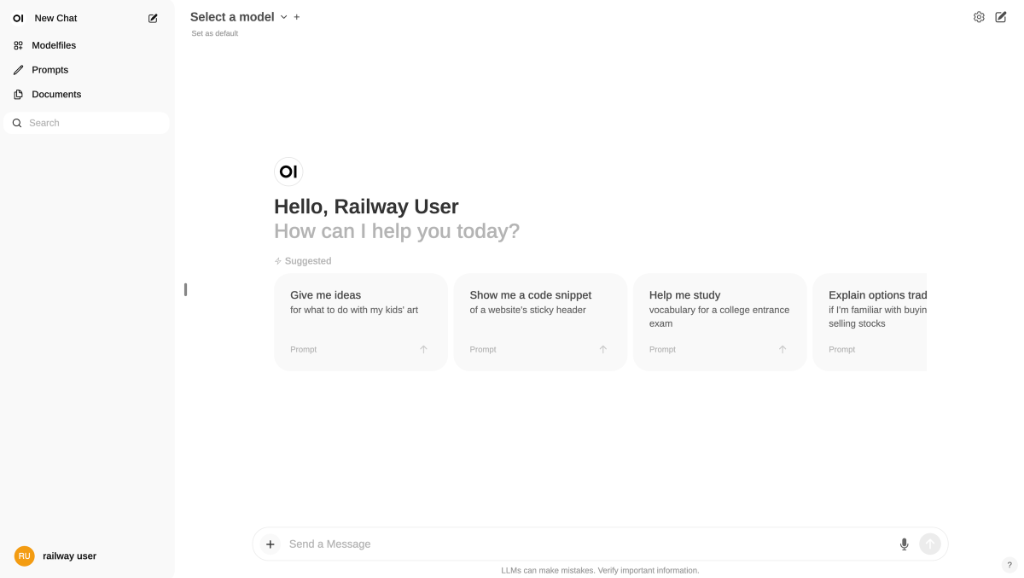
\includegraphics[width=\textwidth]{figures/search_chatgpt.png}\\
\small ChatGPT - AI-powered conversational search
\end{center}
\end{column}
\begin{column}{0.48\textwidth}
\begin{center}
\textbf{E-Commerce Search}\\[0.5em]
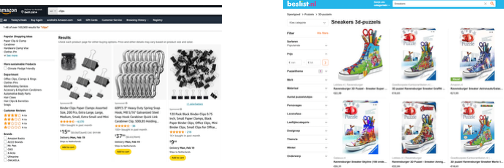
\includegraphics[width=\textwidth]{figures/search_amazon.png}\\
\small Amazon - Product search and recommendations
\end{center}
\end{column}
\end{columns}

\vspace{1em}
\begin{alertblock}{Common Thread}
All search systems share the same core challenge: finding relevant items from massive collections in real-time.
\end{alertblock}
\end{frame}

\begin{frame}{Real-World IR Applications}
\begin{columns}
\begin{column}{0.48\textwidth}
\textbf{Web Search}
\begin{itemize}
    \item Google, Bing, DuckDuckGo
    \item Billions of web pages
    \item Sub-second response time
\end{itemize}
\cpause
\vspace{1em}

\textbf{Enterprise Search}
\begin{itemize}
    \item Search company documents
    \item Email search
    \item Knowledge management
\end{itemize}
\cpause
\end{column}

\begin{column}{0.48\textwidth}
\textbf{E-commerce}
\begin{itemize}
    \item Amazon product search
    \item eBay, Etsy
    \item Recommendation systems
\end{itemize}
\cpause
\vspace{1em}

\textbf{Specialized Domains}
\begin{itemize}
    \item Legal document search (LexisNexis)
    \item Academic papers (Google Scholar)
    \item Medical records (PubMed)
    \item News archives
\end{itemize}
\end{column}
\end{columns}

\vspace{1em}

\begin{center}
\textbf{IR is everywhere you search for information!}
\end{center}
\end{frame}

% ====================================================================
% SECTION: CHALLENGES IN IR
% ====================================================================
\section{Challenges in IR}
\begin{frame}
  \centering
  \LARGE \textbf{Challenges in IR}
\end{frame}

\begin{frame}[shrink]{The Retrieval Challenge: Understanding Intent}
\begin{center}
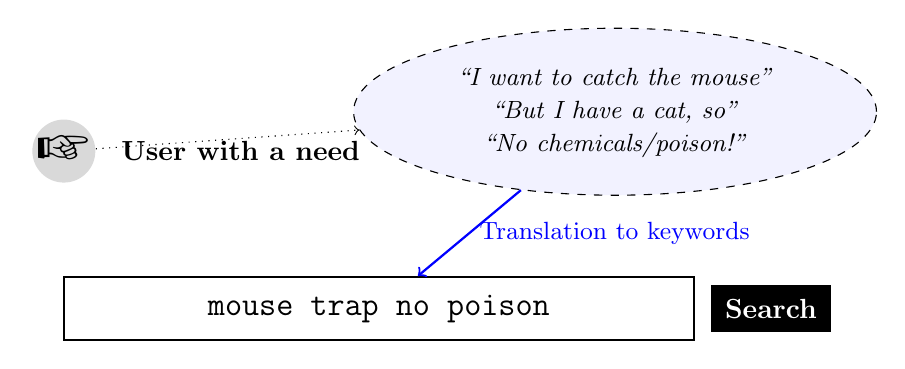
\begin{tikzpicture}[
    searchbox/.style={rectangle, draw, thick, minimum width=8cm, minimum height=0.8cm, font=\large},
    user/.style={circle, fill=gray!30, minimum size=0.8cm},
    icon/.style={font=\huge}
]
    % User Icon
    \node[user] (u) at (0,3) {};
    \node[icon] at (u) {\ding{43}}; % Hand/User representation
    \node[right=0.2cm of u] {\textbf{User with a need}};

    % Search Box
    \node[searchbox, fill=white] (box) at (4,1) {\texttt{mouse trap no poison}};
    \node[right=0.2cm of box, fill=black, text=white, inner sep=5pt] {\textbf{Search}};
    
    % Cloud / Intent
    \node[draw, ellipse, dashed, fill=blue!5, minimum width=4cm, minimum height=1.5cm] (intent) at (7,3.5) {
        \begin{tabular}{c}
            \small \textit{``I want to catch the mouse''} \\
            \small \textit{``But I have a cat, so''} \\
            \small \textit{``No chemicals/poison!''}
        \end{tabular}
    };
    \draw[->, dotted] (u) -- (intent);
    \draw[->, thick, blue] (intent) -- (box) node[midway, right] {\small Translation to keywords};
\end{tikzpicture}
\end{center}

\vspace{1em}
\begin{exampleblock}{The Semantic Gap}
\begin{itemize}
    \item \textbf{Syntactic match:} Docs containing ``mouse'', ``trap'', ``poison''.
    \item \textbf{User intent:} Docs describing \textit{humane} traps or \textit{mechanical} traps.
    \item \textbf{Danger:} Returning docs about ``how poison traps work'' (contains keywords!).
\end{itemize}
\end{exampleblock}
\end{frame}

\begin{frame}[shrink=5]{The Scale of Modern IR}
\begin{block}{Web Search Statistics (2024)}
\begin{itemize}
    \item \textbf{Google:} Processes 8.5+ billion searches per day
    \item \textbf{Index size:} 100+ trillion web pages indexed
    \item \textbf{Freshness:} New pages indexed within hours
    \item \textbf{Speed:} Results in $< 0.5$ seconds on average
\end{itemize}
\cpause
\end{block}
\vspace{1em}

\begin{exampleblock}{Challenges at Scale}
\begin{itemize}
    \item \textbf{Storage:} How to store 100 trillion documents?
    \item \textbf{Speed:} How to search in milliseconds?
    \item \textbf{Relevance:} How to rank billions of results?
    \item \textbf{Freshness:} How to keep index up-to-date?
    \item \textbf{Quality:} How to fight spam and misinformation?
\end{itemize}
\end{exampleblock}
\end{frame}

\begin{frame}[shrink=10]{The Information Retrieval Problem}
\begin{center}
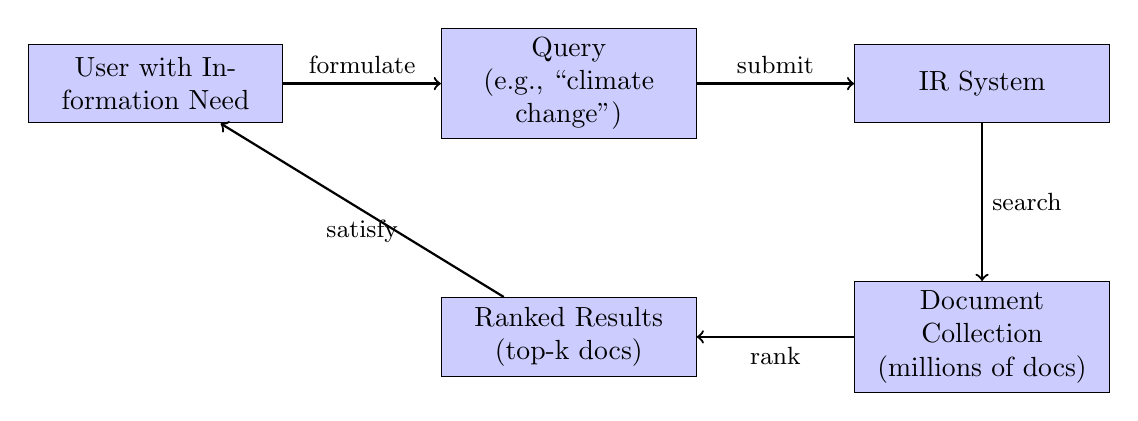
\begin{tikzpicture}[
    node distance=2cm,
    box/.style={rectangle, draw, fill=blue!20, text width=3cm, align=center, minimum height=1cm},
    arrow/.style={->, thick}
]
    \node[box] (user) {User with Information Need};
    \node[box, right=of user] (query) {Query \\ (e.g., ``climate change'')};
    \node[box, right=of query] (system) {IR System};
    \node[box, below=of system] (collection) {Document Collection \\ (millions of docs)};
    \node[box, left=of collection] (results) {Ranked Results \\ (top-k docs)};
    
    \draw[arrow] (user) -- (query) node[midway, above] {\small formulate};
    \draw[arrow] (query) -- (system) node[midway, above] {\small submit};
    \draw[arrow] (system) -- (collection) node[midway, right] {\small search};
    \draw[arrow] (collection) -- (results) node[midway, below] {\small rank};
    \draw[arrow] (results) -- (user) node[midway, below] {\small satisfy};
\end{tikzpicture}
\end{center}

\vspace{1em}
\cpause

\textbf{Core Questions:}
\begin{enumerate}
    \item How to represent documents and queries?
    \item How to match queries to documents efficiently?
    \item How to rank documents by relevance?
\end{enumerate}

\end{frame}

% ====================================================================
% ====================================================================
% SECTION 2: THE IR PROCESS (MOVED TO LECTURE 2)
% ====================================================================
\section{The Information Retrieval Process}
\begin{frame}{The Information Retrieval Process}
\begin{alertblock}{Forward Reference: Lecture 2}
\textbf{The fundamental IR process}, including pipeline architectures and preprocessing, is now covered in detail in \textbf{Lecture 2: Indexing}.
\end{alertblock}

\vspace{1em}
\begin{exampleblock}{Why the change?}
\begin{itemize}
    \item Better logical flow: Preprocessing is tightly coupled with building indexes.
    \item Focus for today: Understanding the models (Boolean and Vector Space).
\end{itemize}
\end{exampleblock}

\vspace{1em}
\begin{center}
\textit{Proceeding to Section 3: Boolean Retrieval...}
\end{center}
\end{frame}

% ====================================================================
% SECTION 3: BOOLEAN RETRIEVAL
% ====================================================================
\section{Boolean Retrieval}
\begin{frame}
  \centering
  \LARGE \textbf{Boolean Retrieval}
\end{frame}


\begin{frame}[shrink=5]{Boolean Retrieval Model}
\begin{block}{Definition}
Documents are retrieved if they satisfy a Boolean expression of query terms
\end{block}
\cpause
\vspace{1em}

\textbf{Boolean Operators:}
\begin{itemize}
    \item \textbf{AND:} Both terms must appear (intersection)
    \item \textbf{OR:} Either term must appear (union)
    \item \textbf{NOT:} Term must not appear (negation)
\end{itemize}
\cpause
\vspace{1em}

\begin{exampleblock}{Example Queries}
\begin{itemize}
    \item \texttt{climate AND change} → docs containing both ``climate'' and ``change''
    \item \texttt{cat OR dog} → docs containing ``cat'' or ``dog'' or both
    \item \texttt{java NOT coffee} → docs with ``java'' but not ``coffee''
    \item \texttt{(climate AND change) OR (global AND warming)}
\end{itemize}
% \cpause
\end{exampleblock}
% \cpause
\end{frame}

\begin{frame}{Boolean Retrieval with Sets}
\textbf{Documents as Sets of Terms}

\vspace{1em}

\begin{columns}
\begin{column}{0.48\textwidth}
\textbf{Document Collection:}
\begin{itemize}
    \item D1: \{cat, sat, mat\}
    \item D2: \{dog, sat, log\}
    \item D3: \{cat, dog, run\}
    \item D4: \{bird, fly, sky\}
\end{itemize}
\cpause
\end{column}

\begin{column}{0.48\textwidth}
\textbf{Inverted Index:}
\begin{itemize}
    \item cat: \{D1, D3\}
    \item dog: \{D2, D3\}
    \item sat: \{D1, D2\}
    \item run: \{D3\}
\end{itemize}
\cpause
\end{column}
\end{columns}

\vspace{1em}

\textbf{Query Processing:}
\begin{itemize}
    \item \texttt{cat AND dog}: \{D1, D3\} $\cap$ \{D2, D3\} = \{D3\}
    \item \texttt{cat OR dog}: \{D1, D3\} $\cup$ \{D2, D3\} = \{D1, D2, D3\}
    \item \texttt{cat NOT dog}: \{D1, D3\} - \{D2, D3\} = \{D1\}
\end{itemize}
% \cpause
\end{frame}

\begin{frame}[shrink=10]{Boolean Retrieval Example}
\textbf{Query:} \texttt{(cat AND mat) OR dog}

\vspace{1em}

\begin{center}
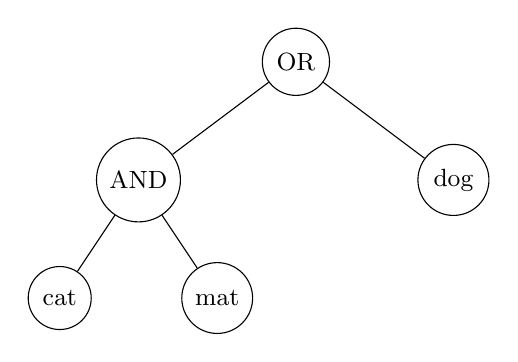
\begin{tikzpicture}[
    level distance=1.5cm,
    level 1/.style={sibling distance=4cm},
    level 2/.style={sibling distance=2cm},
    every node/.style={circle, draw, minimum size=0.8cm, font=\small}
]
    \node {OR}
        child {node {AND}
            child {node {cat}}
            child {node {mat}}
        }
        child {node {dog}};
\end{tikzpicture}
\end{center}

\vspace{1em}

\textbf{Execution:}
\begin{enumerate}
    \item \texttt{cat}: \{D1, D3\}
    \item \texttt{mat}: \{D1\}
    \item \texttt{cat AND mat}: \{D1, D3\} $\cap$ \{D1\} = \{D1\}
    \item \texttt{dog}: \{D2, D3\}
    \cpause
    \item \texttt{(cat AND mat) OR dog}: \{D1\} $\cup$ \{D2, D3\} = \{D1, D2, D3\}
\end{enumerate}
% \cpause
\end{frame}

\begin{frame}[shrink=10]{Advantages of Boolean Retrieval}
\begin{block}{\checkmark Advantages}
\begin{itemize}
    \item[\checkmark] \textbf{Precise control:} Users specify exactly what they want
    \item[\checkmark] \textbf{Transparent:} Clear why documents matched
    \item[\checkmark] \textbf{Efficient:} Fast set operations on posting lists
    \item[\checkmark] \textbf{Predictable:} Same query always returns same results
    \item[\checkmark] \textbf{Expressive:} Can construct complex queries
\end{itemize}
\cpause
\end{block}
% \cpause
\vspace{1em}

\begin{exampleblock}{Use Cases}
\begin{itemize}
    \item Legal document search (very precise requirements)
    \item Patent search (need exact specifications)
    \item Database-like queries on text
    \item Expert users who know what they want
\end{itemize}
% \cpause
\end{exampleblock}
% \cpause
\end{frame}

\begin{frame}{Limitations of Boolean Retrieval}
\begin{alertblock}{\ding{55} Critical Limitations}
\begin{enumerate}
    \item[\ding{55}] \textbf{No ranking}
    \begin{itemize}
        \item All matching documents equally relevant
        \item Can't distinguish ``very relevant'' from ``barely relevant''
    \end{itemize}
\cpause
    \item[\ding{55}] \textbf{All or nothing}
    \begin{itemize}
        \item \texttt{climate AND change AND effects}: No results if one term missing
        \item Too restrictive or too permissive
    \end{itemize}
\cpause
    \item[\ding{55}] \textbf{Hard to formulate queries}
    \begin{itemize}
        \item Most users don't know Boolean operators
        \item Hard to express fuzzy information needs
    \end{itemize}
\cpause
    \item[\ding{55}] \textbf{Result set size unpredictable}
    \begin{itemize}
        \item Could return 0 results or 10 million
        \item Users want ``top 10'', not ``all matching''
    \end{itemize}
% \cpause
\end{enumerate}
% \cpause
\end{alertblock}
% \cpause
\end{frame}

\begin{frame}{Boolean Retrieval: The Feast or Famine Problem}
\begin{columns}
\begin{column}{0.48\textwidth}
\textbf{Too Restrictive (Famine)}
\begin{itemize}
    \item Query: \texttt{machine AND learning AND neural AND networks}
    \item Result: 0 documents
    \item Problem: One term missing kills entire result
\end{itemize}
\cpause
\vspace{1em}

\textbf{Solution?}
\begin{itemize}
    \item User tries: \texttt{machine AND learning}
\end{itemize}
\cpause
\end{column}

\begin{column}{0.48\textwidth}
\textbf{Too Permissive (Feast)}
\begin{itemize}
    \item Query: \texttt{machine AND learning}
    \item Result: 1,000,000 documents
    \item Problem: Which 10 should I read?
\end{itemize}
\cpause
\vspace{1em}

\textbf{Need:}
\begin{itemize}
    \item Ranking by relevance
    \item Graceful degradation
    \item Better matching
\end{itemize}
% \cpause
\end{column}
\end{columns}

\vspace{1em}

\begin{center}
\textbf{This motivates the Vector Space Model!}
\end{center}
\end{frame}

% ====================================================================
% SECTION 4: VECTOR SPACE MODEL
% ====================================================================
\section{The Vector Space Model}
\begin{frame}
  \centering
  \LARGE \textbf{The Vector Space Model}
\end{frame}


\begin{frame}[shrink=10]{From Boolean to Vector Space}
\begin{block}{Key Insight}
Instead of documents being sets of terms (in/out), represent them as \textbf{vectors} with weights for each term
\end{block}
\cpause
\vspace{1em}

\begin{columns}
\begin{column}{0.48\textwidth}
\textbf{Boolean Model:}
\begin{itemize}
    \item D1: \{cat, dog\}
    \item D2: \{cat, mat\}
    \item Binary: term present or not
\end{itemize}
\cpause
\vspace{1em}

\textbf{Query:} \texttt{cat AND dog}
\begin{itemize}
    \item Result: \{D1\}
    \item D2 excluded (no ``dog'')
\end{itemize}
\cpause
\end{column}

\begin{column}{0.48\textwidth}
\textbf{Vector Space Model:}
\begin{itemize}
    \item D1: [cat: 0.5, dog: 0.5, mat: 0]
    \item D2: [cat: 0.7, dog: 0, mat: 0.3]
    \item Weighted: importance/frequency
\end{itemize}
\cpause
\vspace{1em}

\textbf{Query:} [cat: 0.5, dog: 0.5]
\begin{itemize}
    \item Similarity(D1, Q) = 0.5
    \item Similarity(D2, Q) = 0.35
    \item \textbf{Ranked:} D1, then D2
\end{itemize}
\cpause
\end{column}
\end{columns}

\vspace{1em}

\begin{exampleblock}{Advantage}
D2 still returned (has ``cat''), just ranked lower than D1
\end{exampleblock}
% \cpause
\end{frame}

\begin{frame}[shrink=10]{Vector Space Model: Geometric View}
\textbf{Documents and queries as vectors in term space}

\vspace{1em}

\begin{center}
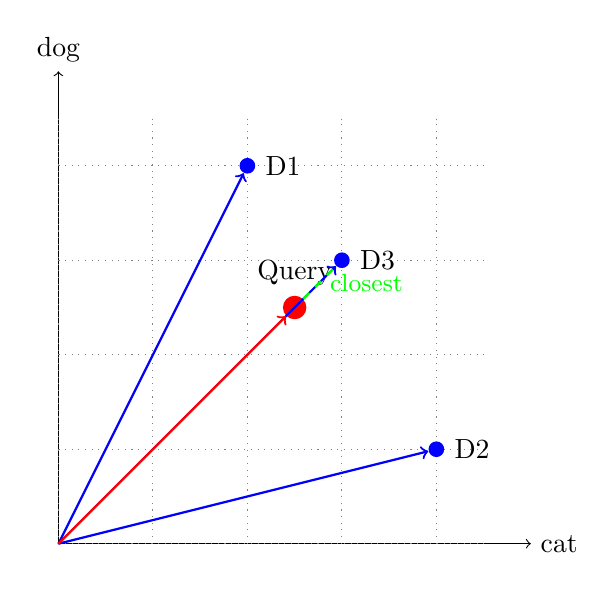
\begin{tikzpicture}[scale=1.2]
    % Axes
    \draw[->] (0,0) -- (5,0) node[right] {cat};
    \draw[->] (0,0) -- (0,5) node[above] {dog};
    
    % Grid
    \draw[gray, dotted] (0,0) grid (4.5,4.5);
    
    % Documents
    \node[circle, fill=blue, inner sep=2pt, label=right:D1] (d1) at (2,4) {};
    \node[circle, fill=blue, inner sep=2pt, label=right:D2] (d2) at (4,1) {};
    \node[circle, fill=blue, inner sep=2pt, label=right:D3] (d3) at (3,3) {};
    
    % Query
    \node[circle, fill=red, inner sep=3pt, label=above:Query] (q) at (2.5,2.5) {};
    
    % Vectors
    \draw[->, thick, blue] (0,0) -- (d1);
    \draw[->, thick, blue] (0,0) -- (d2);
    \draw[->, thick, blue] (0,0) -- (d3);
    \draw[->, thick, red] (0,0) -- (q);
    
    % Similarity illustration
    \draw[dashed, green, thick] (q) -- (d3) node[midway, right] {\small closest};
\end{tikzpicture}
\end{center}

\textbf{Similarity = Angle between vectors} \\
\small (Smaller angle = more similar)
\end{frame}

\begin{frame}[shrink=10]{Term Weighting in Vector Space Model}
\textbf{Question:} How to assign weights to terms?

\vspace{1em}

\begin{block}{Option 1: Binary Weights}
$$w_{t,d} = \begin{cases} 1 & \text{if term } t \text{ appears in doc } d \\ 0 & \text{otherwise} \end{cases}$$
\begin{itemize}
    \item Simple but ignores frequency
\end{itemize}
\cpause
\end{block}
\cpause
\begin{block}{Option 2: Term Frequency (TF)}
$$w_{t,d} = \text{count}(t, d)$$
\begin{itemize}
    \item Better: reflects importance
    \item Problem: Common words get high weight
\end{itemize}
\cpause
\end{block}
\cpause
\begin{alertblock}{Problem with Raw TF}
Document mentioning ``the'' 100 times doesn't make it about ``the''
\end{alertblock}
\cpause
\end{frame}

\begin{frame}[shrink=10]{TF-IDF Weighting}
\textbf{Idea:} Balance term frequency with term rarity

\vspace{1em}

\begin{block}{TF-IDF Formula}
$$w_{t,d} = \text{tf}(t,d) \times \text{idf}(t)$$

where:
\begin{itemize}
    \item $\text{tf}(t,d) = \text{count}(t,d)$ (term frequency in document)
    \item $\text{idf}(t) = \log\frac{N}{\text{df}(t)}$ (inverse document frequency)
    \item $N$ = total number of documents
    \item $\text{df}(t)$ = number of documents containing term $t$
\end{itemize}
\cpause
\end{block}
\cpause
\vspace{1em}

\textbf{Intuition:}
\begin{itemize}
    \item \textbf{High TF:} Term appears often in this document → important for this doc
    \item \textbf{High IDF:} Term is rare across collection → discriminative
    \item \textbf{High TF-IDF:} Important AND discriminative
\end{itemize}
% \cpause
\end{frame}

\begin{frame}[shrink=10]{TF-IDF Example}
\textbf{Collection:} 10,000 documents

\vspace{1em}

\begin{table}
\centering
\small
\begin{tabular}{lcccc}
\toprule
\textbf{Term} & \textbf{tf(t,d)} & \textbf{df(t)} & \textbf{idf(t)} & \textbf{tf-idf} \\
\midrule
neural & 5 & 100 & $\log(10000/100) = 2.0$ & 10.0 \\
network & 3 & 500 & $\log(10000/500) = 1.3$ & 3.9 \\
the & 50 & 9000 & $\log(10000/9000) = 0.05$ & 2.5 \\
\bottomrule
\end{tabular}
\end{table}

\vspace{1em}

\textbf{Observations:}
\begin{itemize}
    \item ``neural'' appears less than ``the'' (5 vs. 50) but gets higher weight (10.0 vs. 2.5)
    \item Rare, discriminative terms weighted higher
    \item Common words automatically downweighted
\end{itemize}
\cpause
\vspace{0.5em}

\begin{alertblock}{Note}
This is a simplified version; we'll cover refined TF-IDF and BM25 in Lecture 3
\end{alertblock}
\cpause
\end{frame}

\begin{frame}[shrink=10]{Document Vectors with TF-IDF}
\textbf{Example Collection:}
\begin{itemize}
    \item D1: ``cat cat dog''
    \item D2: ``cat mat''
    \item D3: ``dog bird bird''
\end{itemize}
\cpause
\vspace{1em}

\textbf{Vocabulary:} \{cat, dog, mat, bird\}

\vspace{1em}

\begin{table}
\centering
\small
\begin{tabular}{lcccc}
\toprule
\textbf{Doc} & \textbf{cat} & \textbf{dog} & \textbf{mat} & \textbf{bird} \\
\midrule
D1 & 2 × log(3/2) = 0.35 & 1 × log(3/2) = 0.18 & 0 & 0 \\
D2 & 1 × log(3/2) = 0.18 & 0 & 1 × log(3/1) = 0.48 & 0 \\
D3 & 0 & 1 × log(3/2) = 0.18 & 0 & 2 × log(3/1) = 0.95 \\
\bottomrule
\end{tabular}
\end{table}

\vspace{1em}

\textbf{Vector Representation:}
\begin{itemize}
    \item D1: [0.35, 0.18, 0, 0]
    \item D2: [0.18, 0, 0.48, 0]
    \item D3: [0, 0.18, 0, 0.95]
\end{itemize}
% \cpause
\end{frame}

\begin{frame}[shrink=10]{Cosine Similarity}
\textbf{How to measure similarity between vectors?}

\vspace{1em}

\begin{block}{Cosine Similarity Formula}
$$\text{sim}(\vec{q}, \vec{d}) = \frac{\vec{q} \cdot \vec{d}}{|\vec{q}| \times |\vec{d}|} = \frac{\sum_{t} q_t \times d_t}{\sqrt{\sum_{t} q_t^2} \times \sqrt{\sum_{t} d_t^2}}$$
\end{block}
\cpause
\vspace{1em}

\textbf{Properties:}
\begin{itemize}
    \item Range: [-1, 1] (or [0, 1] for positive weights)
    \item 1 = identical vectors (same direction)
    \item 0 = orthogonal (no common terms)
    \item -1 = opposite vectors (not relevant for IR)
\end{itemize}
\cpause
\vspace{1em}

\textbf{Why cosine instead of dot product?}
\begin{itemize}
    \item Cosine normalizes for document length
    \item Long documents don't automatically score higher
\end{itemize}
% \cpause
\end{frame}

\begin{frame}[shrink=10]{Cosine Similarity: Example Calculation}
\textbf{Query:} ``cat dog'' → $\vec{q} = [0.5, 0.5, 0, 0]$ \\
\textbf{Documents:}
\begin{itemize}
    \item D1: [0.35, 0.18, 0, 0]
    \item D2: [0.18, 0, 0.48, 0]
    \item D3: [0, 0.18, 0, 0.95]
\end{itemize}
\cpause
\vspace{1em}

\textbf{Similarity Calculations:}

\begin{align*}
\text{sim}(q, D1) &= \frac{(0.5 \times 0.35) + (0.5 \times 0.18)}{\sqrt{0.5^2 + 0.5^2} \times \sqrt{0.35^2 + 0.18^2}} \\
&= \frac{0.265}{0.707 \times 0.394} = 0.95 \\
\text{sim}(q, D2) &= \frac{0.5 \times 0.18}{0.707 \times 0.511} = 0.25 \\
\text{sim}(q, D3) &= \frac{0.5 \times 0.18}{0.707 \times 0.967} = 0.13
\end{align*}

\vspace{1em}

\textbf{Ranking:} D1 (0.95)  >  D2 (0.25)  >  D3 (0.13)
\end{frame}

\begin{frame}{VSM vs. Boolean Retrieval}
\begin{table}
\centering
\small
\begin{tabular}{lll}
\toprule
\textbf{Aspect} & \textbf{Boolean} & \textbf{Vector Space} \\
\midrule
Matching & Exact (in/out) & Partial (weighted) \\
Ranking & No & Yes (by similarity) \\
Result size & Unpredictable & Top-$k$ \\
Term weighting & Binary & TF-IDF \\
Query expression & Boolean operators & Term list \\
Robustness & Brittle & Graceful degradation \\
User friendliness & Expert users & General users \\
Relevance & All equal & Ranked by relevance \\
\bottomrule
\end{tabular}
\end{table}

\vspace{1em}

\begin{block}{Modern Usage}
\begin{itemize}
    \item \textbf{Boolean:} Still used in legal, patent search (precision critical)
    \item \textbf{Vector Space:} Foundation for web search, most IR systems
    \item \textbf{Hybrid:} Many systems combine both approaches
\end{itemize}
\cpause
\end{block}
\cpause
\end{frame}

\begin{frame}[shrink=5]{Advantages of Vector Space Model}
\begin{block}{\checkmark Key Advantages}
\begin{enumerate}
    \item \textbf{Ranking by relevance}
    \begin{itemize}
        \item Documents ordered by similarity to query
        \item Users get best results first
    \end{itemize}
\cpause
    \item \textbf{Partial matching}
    \begin{itemize}
        \item Documents matching some query terms still retrieved
        \item Graceful degradation (no feast/famine)
    \end{itemize}
\cpause
    \item \textbf{Term weighting}
    \begin{itemize}
        \item Important terms weighted higher (TF-IDF)
        \item Automatic handling of common words
    \end{itemize}
\cpause
    \item \textbf{Simple queries}
    \begin{itemize}
        \item Users just type terms (no Boolean operators)
        \item Natural for web search
    \end{itemize}
\cpause
    \item \textbf{Tunable}
    \begin{itemize}
        \item Can adjust weighting schemes
        \item Foundation for more advanced models (BM25, Lecture 3)
    \end{itemize}
\cpause
\end{enumerate}
\end{block}
\end{frame}

\begin{frame}[shrink=10]{Limitations of Vector Space Model}
\begin{alertblock}{\ding{55} Limitations}
\begin{enumerate}
    \item \textbf{Bag of words assumption}
    \begin{itemize}
        \item Word order ignored: ``dog bites man'' = ``man bites dog''
        \item No phrase matching
    \end{itemize}
\cpause
    \item \textbf{Term independence}
    \begin{itemize}
        \item Assumes terms are independent
        \item ``New York'' treated as ``New'' and ``York''
    \end{itemize}
\cpause
    \item \textbf{Synonymy}
    \begin{itemize}
        \item ``car'' and ``automobile'' treated as different
        \item Misses relevant documents with synonyms
    \end{itemize}
\cpause
    \item \textbf{Polysemy}
    \begin{itemize}
        \item ``bank'' (financial) vs. ``bank'' (river) undistinguished
        \item Can retrieve irrelevant documents
    \end{itemize}

\end{enumerate}

\end{alertblock}

\end{frame}


% ====================================================================
% SECTION 7: CONNECTIONS TO FUTURE LECTURES
% ====================================================================
\section{Questions}
\begin{frame}
  \centering
  \LARGE \textbf{Looking Ahead}
\end{frame}



\end{document}" for static version
% ====================================================================
\newif\ifanimated
\animatedtrue
\ifdefined\staticmode
  \animatedfalse
\fi

% Conditional pause command
\newcommand{\cpause}{\ifanimated\pause\fi}

% Packages
\usepackage{amsmath}
\usepackage{amssymb}
\usepackage{pifont} % For checkmarks and crosses if needed
\usepackage{amssymb}
\usepackage{algorithm}
\usepackage{algorithmic}
\usepackage{graphicx}
\usepackage{tikz}
\usepackage{booktabs}
\usepackage{listings}
\usepackage{xcolor}

% Python code styling
\lstset{
    language=Python,
    basicstyle=\ttfamily\footnotesize,
    keywordstyle=\color{blue},
    commentstyle=\color{gray},
    stringstyle=\color{red},
    showstringspaces=false,
    breaklines=true,
    frame=single,
    numbers=left,
    numberstyle=\tiny\color{gray}
}

% TikZ libraries
\usetikzlibrary{shapes,arrows,positioning,calc,patterns}

% Title information
\title[Introduction to IR]{Information Retrieval Introduction}
\subtitle{Lecture 1: Vector Space Model \& Boolean Retrieval}
\author{Avishek Anand}
\institute{Information Retrieval}
\date{\today}

\begin{document}

% Title slide
\begin{frame}
\titlepage
\end{frame}

% Course Overview
\begin{frame}{Course Overview}
\begin{enumerate}
    \item \textbf{Introduction to IR: Vector Space Model \& Boolean Retrieval} $\leftarrow$ Today
    \item Indexing: Sparse and Dense
    \item Query Understanding \& Expansion
    \item Evaluation of IR Systems
    \item Ranking: BM25, Language Models, and Beyond
    \item Embeddings \& Neural Ranking
    \item Dense Retrieval
    \item Learning to Rank
    \item Recommender Systems
    \item Retrieval Augmented Generation (RAG)
    \item LLMs as a Judge
\end{enumerate}
\cpause
\vspace{1em}
\textbf{Today's Goals:}
\begin{itemize}
    \item Understand what IR is and why it matters
    \item Learn the fundamental IR process
    \item Master Boolean retrieval and the vector space model
    % \item Build your first search engine
\end{itemize}
\end{frame}

\begin{frame}{Outline}
\tableofcontents
\end{frame}

% ====================================================================
% SECTION 1: WHAT IS INFORMATION RETRIEVAL?
% ====================================================================
\section{What is Information Retrieval?}
\begin{frame}
  \centering
  \LARGE \textbf{What is Information Retrieval?}
\end{frame}


\begin{frame}{What is Information Retrieval?}
\begin{block}{Definition}
Information Retrieval (IR) is finding material (usually documents) of an unstructured nature (usually text) that satisfies an information need from within large collections (usually stored on computers).
\end{block}
\cpause
\vspace{1em}

\begin{exampleblock}{The Essence of IR: Given an Information Need}
\begin{itemize}
    \item \textbf{Find relevant results} that satisfy the information need
    \item \textbf{By searching over a large collection} of items (billions of documents)
    \item \textbf{In reasonable time:}
    \begin{itemize}
        \item Web search: $< 1$ second
        \item AI/conversational systems: allow more time for generation
    \end{itemize}
    \item \textbf{Present results} in a manner that is easily consumable by humans
\end{itemize}
\end{exampleblock}
\end{frame}


\begin{frame}{IR vs. Database Systems}
\begin{table}
\centering
\begin{tabular}{lll}
\toprule
\textbf{Aspect} & \textbf{Database Systems} & \textbf{IR Systems} \\
\midrule
Data & Structured (tables, schemas) & Unstructured (text, documents) \\
Queries & Precise (SQL) & Vague (natural language) \\
Matching & Exact & Approximate/Ranked \\
Result & All matching records & Top-k relevant documents \\
Failure & No results or all results & Ranked list (best effort) \\
\midrule
Example & \texttt{SELECT * WHERE age>30} & ``climate change effects'' \\
\bottomrule
\end{tabular}
\end{table}

\vspace{1em}
\cpause

\begin{alertblock}{Key Difference}
Databases: \textit{``Give me all records matching X''} \\
IR: \textit{``Give me the most relevant documents about X''}
\end{alertblock}
\end{frame}

\begin{frame}[shrink]{IR vs. Natural Language Processing (NLP)}
\begin{block}{The Relationship}
IR and NLP are closely related but have different focal points:
\end{block}

\begin{columns}
\begin{column}{0.48\textwidth}
\textbf{NLP (Language Centric)}
\begin{itemize}
    \item Focus on language \textbf{understanding}, representation, and \textbf{generation}.
    \item Deep analysis of syntax, semantics, and pragmatics.
    \item Models like BERT, Llama, GPT.
\end{itemize}
\end{column}

\begin{column}{0.48\textwidth}
\textbf{IR (Scale \& Need Centric)}
\begin{itemize}
    \item Focus on \textbf{information seeking} at a massive scale.
    \item Uses NLP tech as a toolkit to model relevance.
    \item Priority: Speed, ranking, and satisfying user needs.
\end{itemize}
\end{column}
\end{columns}

\vspace{0.5em}

\begin{exampleblock}{Typical Tasks}
\begin{itemize}
    \item \textbf{NLP:} Named Entity Recognition, Dependency Parsing, Translation, Summarization.
    \item \textbf{IR:} Web Search, Recommendation Systems, Ad-hoc Retrieval, Question Answering.
\end{itemize}
\end{exampleblock}
\end{frame}


\begin{frame}[shrink=5]{Examples of Search Systems}
\begin{columns}
\begin{column}{0.48\textwidth}
\begin{center}
\textbf{Conversational AI Search}\\[0.5em]
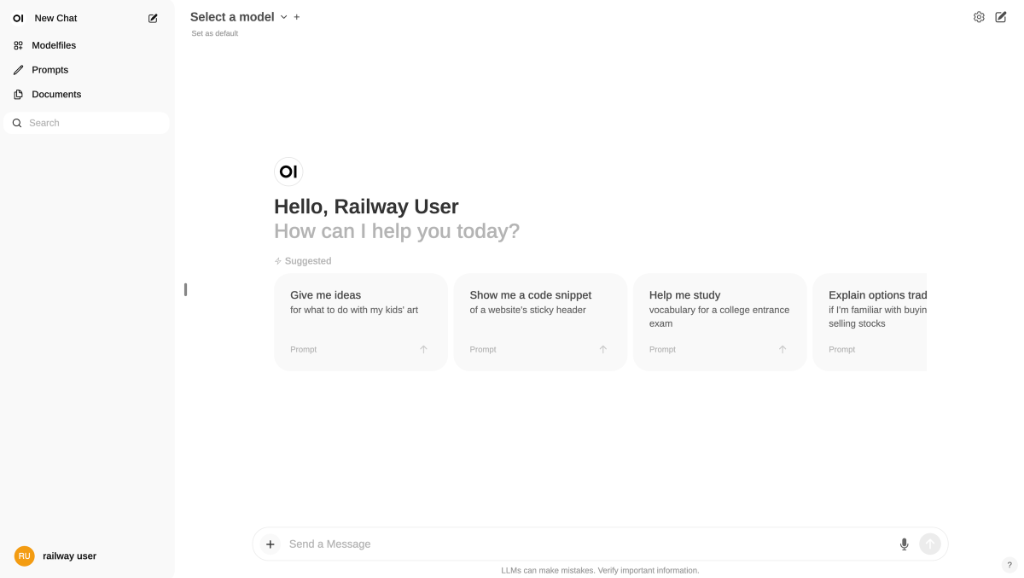
\includegraphics[width=\textwidth]{figures/search_chatgpt.png}\\
\small ChatGPT - AI-powered conversational search
\end{center}
\end{column}
\begin{column}{0.48\textwidth}
\begin{center}
\textbf{E-Commerce Search}\\[0.5em]
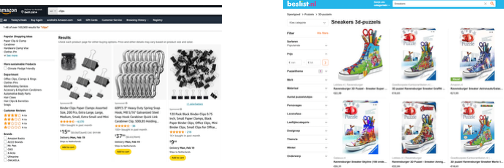
\includegraphics[width=\textwidth]{figures/search_amazon.png}\\
\small Amazon - Product search and recommendations
\end{center}
\end{column}
\end{columns}

\vspace{1em}
\begin{alertblock}{Common Thread}
All search systems share the same core challenge: finding relevant items from massive collections in real-time.
\end{alertblock}
\end{frame}

\begin{frame}{Real-World IR Applications}
\begin{columns}
\begin{column}{0.48\textwidth}
\textbf{Web Search}
\begin{itemize}
    \item Google, Bing, DuckDuckGo
    \item Billions of web pages
    \item Sub-second response time
\end{itemize}
\cpause
\vspace{1em}

\textbf{Enterprise Search}
\begin{itemize}
    \item Search company documents
    \item Email search
    \item Knowledge management
\end{itemize}
\cpause
\end{column}

\begin{column}{0.48\textwidth}
\textbf{E-commerce}
\begin{itemize}
    \item Amazon product search
    \item eBay, Etsy
    \item Recommendation systems
\end{itemize}
\cpause
\vspace{1em}

\textbf{Specialized Domains}
\begin{itemize}
    \item Legal document search (LexisNexis)
    \item Academic papers (Google Scholar)
    \item Medical records (PubMed)
    \item News archives
\end{itemize}
\end{column}
\end{columns}

\vspace{1em}

\begin{center}
\textbf{IR is everywhere you search for information!}
\end{center}
\end{frame}

% ====================================================================
% SECTION: CHALLENGES IN IR
% ====================================================================
\section{Challenges in IR}
\begin{frame}
  \centering
  \LARGE \textbf{Challenges in IR}
\end{frame}

\begin{frame}[shrink]{The Retrieval Challenge: Understanding Intent}
\begin{center}
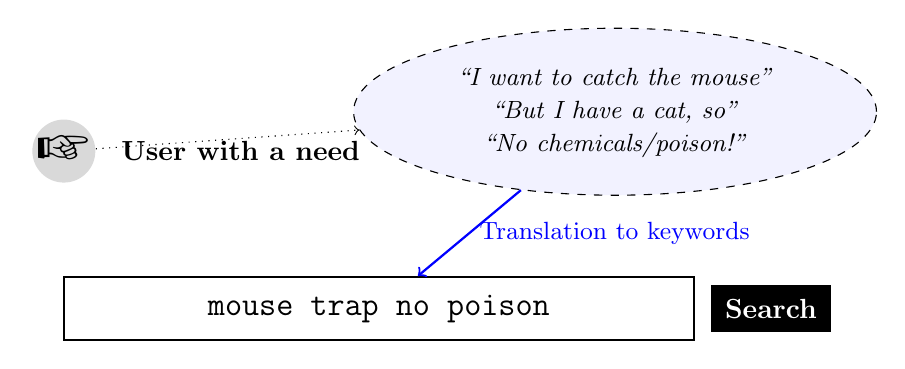
\begin{tikzpicture}[
    searchbox/.style={rectangle, draw, thick, minimum width=8cm, minimum height=0.8cm, font=\large},
    user/.style={circle, fill=gray!30, minimum size=0.8cm},
    icon/.style={font=\huge}
]
    % User Icon
    \node[user] (u) at (0,3) {};
    \node[icon] at (u) {\ding{43}}; % Hand/User representation
    \node[right=0.2cm of u] {\textbf{User with a need}};

    % Search Box
    \node[searchbox, fill=white] (box) at (4,1) {\texttt{mouse trap no poison}};
    \node[right=0.2cm of box, fill=black, text=white, inner sep=5pt] {\textbf{Search}};
    
    % Cloud / Intent
    \node[draw, ellipse, dashed, fill=blue!5, minimum width=4cm, minimum height=1.5cm] (intent) at (7,3.5) {
        \begin{tabular}{c}
            \small \textit{``I want to catch the mouse''} \\
            \small \textit{``But I have a cat, so''} \\
            \small \textit{``No chemicals/poison!''}
        \end{tabular}
    };
    \draw[->, dotted] (u) -- (intent);
    \draw[->, thick, blue] (intent) -- (box) node[midway, right] {\small Translation to keywords};
\end{tikzpicture}
\end{center}

\vspace{1em}
\begin{exampleblock}{The Semantic Gap}
\begin{itemize}
    \item \textbf{Syntactic match:} Docs containing ``mouse'', ``trap'', ``poison''.
    \item \textbf{User intent:} Docs describing \textit{humane} traps or \textit{mechanical} traps.
    \item \textbf{Danger:} Returning docs about ``how poison traps work'' (contains keywords!).
\end{itemize}
\end{exampleblock}
\end{frame}

\begin{frame}[shrink=5]{The Scale of Modern IR}
\begin{block}{Web Search Statistics (2024)}
\begin{itemize}
    \item \textbf{Google:} Processes 8.5+ billion searches per day
    \item \textbf{Index size:} 100+ trillion web pages indexed
    \item \textbf{Freshness:} New pages indexed within hours
    \item \textbf{Speed:} Results in $< 0.5$ seconds on average
\end{itemize}
\cpause
\end{block}
\vspace{1em}

\begin{exampleblock}{Challenges at Scale}
\begin{itemize}
    \item \textbf{Storage:} How to store 100 trillion documents?
    \item \textbf{Speed:} How to search in milliseconds?
    \item \textbf{Relevance:} How to rank billions of results?
    \item \textbf{Freshness:} How to keep index up-to-date?
    \item \textbf{Quality:} How to fight spam and misinformation?
\end{itemize}
\end{exampleblock}
\end{frame}

\begin{frame}[shrink=10]{The Information Retrieval Problem}
\begin{center}
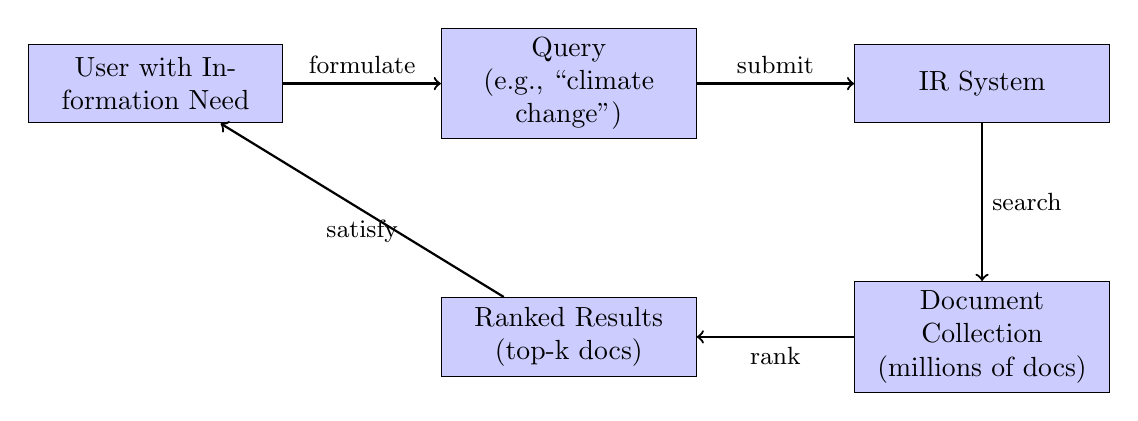
\begin{tikzpicture}[
    node distance=2cm,
    box/.style={rectangle, draw, fill=blue!20, text width=3cm, align=center, minimum height=1cm},
    arrow/.style={->, thick}
]
    \node[box] (user) {User with Information Need};
    \node[box, right=of user] (query) {Query \\ (e.g., ``climate change'')};
    \node[box, right=of query] (system) {IR System};
    \node[box, below=of system] (collection) {Document Collection \\ (millions of docs)};
    \node[box, left=of collection] (results) {Ranked Results \\ (top-k docs)};
    
    \draw[arrow] (user) -- (query) node[midway, above] {\small formulate};
    \draw[arrow] (query) -- (system) node[midway, above] {\small submit};
    \draw[arrow] (system) -- (collection) node[midway, right] {\small search};
    \draw[arrow] (collection) -- (results) node[midway, below] {\small rank};
    \draw[arrow] (results) -- (user) node[midway, below] {\small satisfy};
\end{tikzpicture}
\end{center}

\vspace{1em}
\cpause

\textbf{Core Questions:}
\begin{enumerate}
    \item How to represent documents and queries?
    \item How to match queries to documents efficiently?
    \item How to rank documents by relevance?
\end{enumerate}

\end{frame}

% ====================================================================
% ====================================================================
% SECTION 2: THE IR PROCESS (MOVED TO LECTURE 2)
% ====================================================================
\section{The Information Retrieval Process}
\begin{frame}{The Information Retrieval Process}
\begin{alertblock}{Forward Reference: Lecture 2}
\textbf{The fundamental IR process}, including pipeline architectures and preprocessing, is now covered in detail in \textbf{Lecture 2: Indexing}.
\end{alertblock}

\vspace{1em}
\begin{exampleblock}{Why the change?}
\begin{itemize}
    \item Better logical flow: Preprocessing is tightly coupled with building indexes.
    \item Focus for today: Understanding the models (Boolean and Vector Space).
\end{itemize}
\end{exampleblock}

\vspace{1em}
\begin{center}
\textit{Proceeding to Section 3: Boolean Retrieval...}
\end{center}
\end{frame}

% ====================================================================
% SECTION 3: BOOLEAN RETRIEVAL
% ====================================================================
\section{Boolean Retrieval}
\begin{frame}
  \centering
  \LARGE \textbf{Boolean Retrieval}
\end{frame}


\begin{frame}[shrink=5]{Boolean Retrieval Model}
\begin{block}{Definition}
Documents are retrieved if they satisfy a Boolean expression of query terms
\end{block}
\cpause
\vspace{1em}

\textbf{Boolean Operators:}
\begin{itemize}
    \item \textbf{AND:} Both terms must appear (intersection)
    \item \textbf{OR:} Either term must appear (union)
    \item \textbf{NOT:} Term must not appear (negation)
\end{itemize}
\cpause
\vspace{1em}

\begin{exampleblock}{Example Queries}
\begin{itemize}
    \item \texttt{climate AND change} → docs containing both ``climate'' and ``change''
    \item \texttt{cat OR dog} → docs containing ``cat'' or ``dog'' or both
    \item \texttt{java NOT coffee} → docs with ``java'' but not ``coffee''
    \item \texttt{(climate AND change) OR (global AND warming)}
\end{itemize}
% \cpause
\end{exampleblock}
% \cpause
\end{frame}

\begin{frame}{Boolean Retrieval with Sets}
\textbf{Documents as Sets of Terms}

\vspace{1em}

\begin{columns}
\begin{column}{0.48\textwidth}
\textbf{Document Collection:}
\begin{itemize}
    \item D1: \{cat, sat, mat\}
    \item D2: \{dog, sat, log\}
    \item D3: \{cat, dog, run\}
    \item D4: \{bird, fly, sky\}
\end{itemize}
\cpause
\end{column}

\begin{column}{0.48\textwidth}
\textbf{Inverted Index:}
\begin{itemize}
    \item cat: \{D1, D3\}
    \item dog: \{D2, D3\}
    \item sat: \{D1, D2\}
    \item run: \{D3\}
\end{itemize}
\cpause
\end{column}
\end{columns}

\vspace{1em}

\textbf{Query Processing:}
\begin{itemize}
    \item \texttt{cat AND dog}: \{D1, D3\} $\cap$ \{D2, D3\} = \{D3\}
    \item \texttt{cat OR dog}: \{D1, D3\} $\cup$ \{D2, D3\} = \{D1, D2, D3\}
    \item \texttt{cat NOT dog}: \{D1, D3\} - \{D2, D3\} = \{D1\}
\end{itemize}
% \cpause
\end{frame}

\begin{frame}[shrink=10]{Boolean Retrieval Example}
\textbf{Query:} \texttt{(cat AND mat) OR dog}

\vspace{1em}

\begin{center}
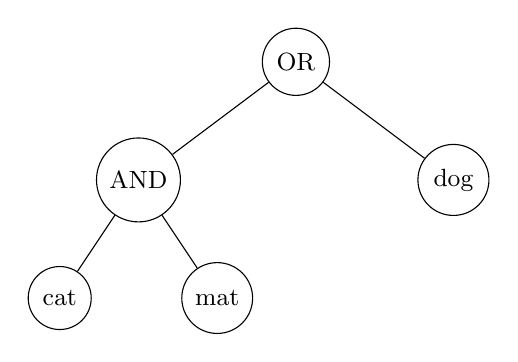
\begin{tikzpicture}[
    level distance=1.5cm,
    level 1/.style={sibling distance=4cm},
    level 2/.style={sibling distance=2cm},
    every node/.style={circle, draw, minimum size=0.8cm, font=\small}
]
    \node {OR}
        child {node {AND}
            child {node {cat}}
            child {node {mat}}
        }
        child {node {dog}};
\end{tikzpicture}
\end{center}

\vspace{1em}

\textbf{Execution:}
\begin{enumerate}
    \item \texttt{cat}: \{D1, D3\}
    \item \texttt{mat}: \{D1\}
    \item \texttt{cat AND mat}: \{D1, D3\} $\cap$ \{D1\} = \{D1\}
    \item \texttt{dog}: \{D2, D3\}
    \cpause
    \item \texttt{(cat AND mat) OR dog}: \{D1\} $\cup$ \{D2, D3\} = \{D1, D2, D3\}
\end{enumerate}
% \cpause
\end{frame}

\begin{frame}[shrink=10]{Advantages of Boolean Retrieval}
\begin{block}{\checkmark Advantages}
\begin{itemize}
    \item[\checkmark] \textbf{Precise control:} Users specify exactly what they want
    \item[\checkmark] \textbf{Transparent:} Clear why documents matched
    \item[\checkmark] \textbf{Efficient:} Fast set operations on posting lists
    \item[\checkmark] \textbf{Predictable:} Same query always returns same results
    \item[\checkmark] \textbf{Expressive:} Can construct complex queries
\end{itemize}
\cpause
\end{block}
% \cpause
\vspace{1em}

\begin{exampleblock}{Use Cases}
\begin{itemize}
    \item Legal document search (very precise requirements)
    \item Patent search (need exact specifications)
    \item Database-like queries on text
    \item Expert users who know what they want
\end{itemize}
% \cpause
\end{exampleblock}
% \cpause
\end{frame}

\begin{frame}{Limitations of Boolean Retrieval}
\begin{alertblock}{\ding{55} Critical Limitations}
\begin{enumerate}
    \item[\ding{55}] \textbf{No ranking}
    \begin{itemize}
        \item All matching documents equally relevant
        \item Can't distinguish ``very relevant'' from ``barely relevant''
    \end{itemize}
\cpause
    \item[\ding{55}] \textbf{All or nothing}
    \begin{itemize}
        \item \texttt{climate AND change AND effects}: No results if one term missing
        \item Too restrictive or too permissive
    \end{itemize}
\cpause
    \item[\ding{55}] \textbf{Hard to formulate queries}
    \begin{itemize}
        \item Most users don't know Boolean operators
        \item Hard to express fuzzy information needs
    \end{itemize}
\cpause
    \item[\ding{55}] \textbf{Result set size unpredictable}
    \begin{itemize}
        \item Could return 0 results or 10 million
        \item Users want ``top 10'', not ``all matching''
    \end{itemize}
% \cpause
\end{enumerate}
% \cpause
\end{alertblock}
% \cpause
\end{frame}

\begin{frame}{Boolean Retrieval: The Feast or Famine Problem}
\begin{columns}
\begin{column}{0.48\textwidth}
\textbf{Too Restrictive (Famine)}
\begin{itemize}
    \item Query: \texttt{machine AND learning AND neural AND networks}
    \item Result: 0 documents
    \item Problem: One term missing kills entire result
\end{itemize}
\cpause
\vspace{1em}

\textbf{Solution?}
\begin{itemize}
    \item User tries: \texttt{machine AND learning}
\end{itemize}
\cpause
\end{column}

\begin{column}{0.48\textwidth}
\textbf{Too Permissive (Feast)}
\begin{itemize}
    \item Query: \texttt{machine AND learning}
    \item Result: 1,000,000 documents
    \item Problem: Which 10 should I read?
\end{itemize}
\cpause
\vspace{1em}

\textbf{Need:}
\begin{itemize}
    \item Ranking by relevance
    \item Graceful degradation
    \item Better matching
\end{itemize}
% \cpause
\end{column}
\end{columns}

\vspace{1em}

\begin{center}
\textbf{This motivates the Vector Space Model!}
\end{center}
\end{frame}

% ====================================================================
% SECTION 4: VECTOR SPACE MODEL
% ====================================================================
\section{The Vector Space Model}
\begin{frame}
  \centering
  \LARGE \textbf{The Vector Space Model}
\end{frame}


\begin{frame}[shrink=10]{From Boolean to Vector Space}
\begin{block}{Key Insight}
Instead of documents being sets of terms (in/out), represent them as \textbf{vectors} with weights for each term
\end{block}
\cpause
\vspace{1em}

\begin{columns}
\begin{column}{0.48\textwidth}
\textbf{Boolean Model:}
\begin{itemize}
    \item D1: \{cat, dog\}
    \item D2: \{cat, mat\}
    \item Binary: term present or not
\end{itemize}
\cpause
\vspace{1em}

\textbf{Query:} \texttt{cat AND dog}
\begin{itemize}
    \item Result: \{D1\}
    \item D2 excluded (no ``dog'')
\end{itemize}
\cpause
\end{column}

\begin{column}{0.48\textwidth}
\textbf{Vector Space Model:}
\begin{itemize}
    \item D1: [cat: 0.5, dog: 0.5, mat: 0]
    \item D2: [cat: 0.7, dog: 0, mat: 0.3]
    \item Weighted: importance/frequency
\end{itemize}
\cpause
\vspace{1em}

\textbf{Query:} [cat: 0.5, dog: 0.5]
\begin{itemize}
    \item Similarity(D1, Q) = 0.5
    \item Similarity(D2, Q) = 0.35
    \item \textbf{Ranked:} D1, then D2
\end{itemize}
\cpause
\end{column}
\end{columns}

\vspace{1em}

\begin{exampleblock}{Advantage}
D2 still returned (has ``cat''), just ranked lower than D1
\end{exampleblock}
% \cpause
\end{frame}

\begin{frame}[shrink=10]{Vector Space Model: Geometric View}
\textbf{Documents and queries as vectors in term space}

\vspace{1em}

\begin{center}
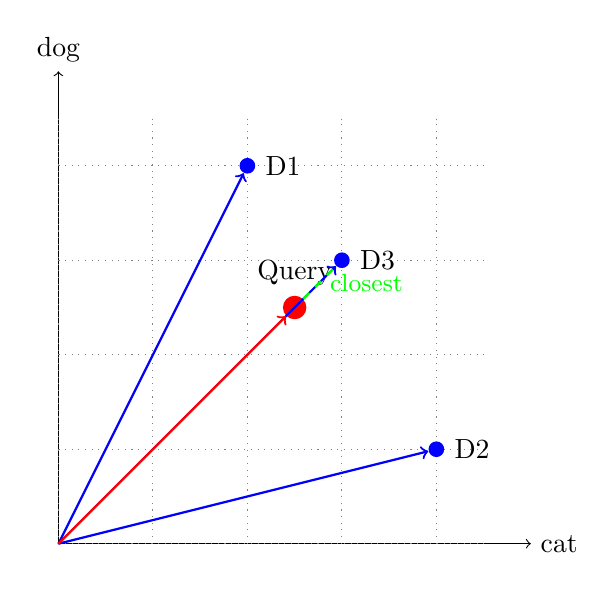
\begin{tikzpicture}[scale=1.2]
    % Axes
    \draw[->] (0,0) -- (5,0) node[right] {cat};
    \draw[->] (0,0) -- (0,5) node[above] {dog};
    
    % Grid
    \draw[gray, dotted] (0,0) grid (4.5,4.5);
    
    % Documents
    \node[circle, fill=blue, inner sep=2pt, label=right:D1] (d1) at (2,4) {};
    \node[circle, fill=blue, inner sep=2pt, label=right:D2] (d2) at (4,1) {};
    \node[circle, fill=blue, inner sep=2pt, label=right:D3] (d3) at (3,3) {};
    
    % Query
    \node[circle, fill=red, inner sep=3pt, label=above:Query] (q) at (2.5,2.5) {};
    
    % Vectors
    \draw[->, thick, blue] (0,0) -- (d1);
    \draw[->, thick, blue] (0,0) -- (d2);
    \draw[->, thick, blue] (0,0) -- (d3);
    \draw[->, thick, red] (0,0) -- (q);
    
    % Similarity illustration
    \draw[dashed, green, thick] (q) -- (d3) node[midway, right] {\small closest};
\end{tikzpicture}
\end{center}

\textbf{Similarity = Angle between vectors} \\
\small (Smaller angle = more similar)
\end{frame}

\begin{frame}[shrink=10]{Term Weighting in Vector Space Model}
\textbf{Question:} How to assign weights to terms?

\vspace{1em}

\begin{block}{Option 1: Binary Weights}
$$w_{t,d} = \begin{cases} 1 & \text{if term } t \text{ appears in doc } d \\ 0 & \text{otherwise} \end{cases}$$
\begin{itemize}
    \item Simple but ignores frequency
\end{itemize}
\cpause
\end{block}
\cpause
\begin{block}{Option 2: Term Frequency (TF)}
$$w_{t,d} = \text{count}(t, d)$$
\begin{itemize}
    \item Better: reflects importance
    \item Problem: Common words get high weight
\end{itemize}
\cpause
\end{block}
\cpause
\begin{alertblock}{Problem with Raw TF}
Document mentioning ``the'' 100 times doesn't make it about ``the''
\end{alertblock}
\cpause
\end{frame}

\begin{frame}[shrink=10]{TF-IDF Weighting}
\textbf{Idea:} Balance term frequency with term rarity

\vspace{1em}

\begin{block}{TF-IDF Formula}
$$w_{t,d} = \text{tf}(t,d) \times \text{idf}(t)$$

where:
\begin{itemize}
    \item $\text{tf}(t,d) = \text{count}(t,d)$ (term frequency in document)
    \item $\text{idf}(t) = \log\frac{N}{\text{df}(t)}$ (inverse document frequency)
    \item $N$ = total number of documents
    \item $\text{df}(t)$ = number of documents containing term $t$
\end{itemize}
\cpause
\end{block}
\cpause
\vspace{1em}

\textbf{Intuition:}
\begin{itemize}
    \item \textbf{High TF:} Term appears often in this document → important for this doc
    \item \textbf{High IDF:} Term is rare across collection → discriminative
    \item \textbf{High TF-IDF:} Important AND discriminative
\end{itemize}
% \cpause
\end{frame}

\begin{frame}[shrink=10]{TF-IDF Example}
\textbf{Collection:} 10,000 documents

\vspace{1em}

\begin{table}
\centering
\small
\begin{tabular}{lcccc}
\toprule
\textbf{Term} & \textbf{tf(t,d)} & \textbf{df(t)} & \textbf{idf(t)} & \textbf{tf-idf} \\
\midrule
neural & 5 & 100 & $\log(10000/100) = 2.0$ & 10.0 \\
network & 3 & 500 & $\log(10000/500) = 1.3$ & 3.9 \\
the & 50 & 9000 & $\log(10000/9000) = 0.05$ & 2.5 \\
\bottomrule
\end{tabular}
\end{table}

\vspace{1em}

\textbf{Observations:}
\begin{itemize}
    \item ``neural'' appears less than ``the'' (5 vs. 50) but gets higher weight (10.0 vs. 2.5)
    \item Rare, discriminative terms weighted higher
    \item Common words automatically downweighted
\end{itemize}
\cpause
\vspace{0.5em}

\begin{alertblock}{Note}
This is a simplified version; we'll cover refined TF-IDF and BM25 in Lecture 3
\end{alertblock}
\cpause
\end{frame}

\begin{frame}[shrink=10]{Document Vectors with TF-IDF}
\textbf{Example Collection:}
\begin{itemize}
    \item D1: ``cat cat dog''
    \item D2: ``cat mat''
    \item D3: ``dog bird bird''
\end{itemize}
\cpause
\vspace{1em}

\textbf{Vocabulary:} \{cat, dog, mat, bird\}

\vspace{1em}

\begin{table}
\centering
\small
\begin{tabular}{lcccc}
\toprule
\textbf{Doc} & \textbf{cat} & \textbf{dog} & \textbf{mat} & \textbf{bird} \\
\midrule
D1 & 2 × log(3/2) = 0.35 & 1 × log(3/2) = 0.18 & 0 & 0 \\
D2 & 1 × log(3/2) = 0.18 & 0 & 1 × log(3/1) = 0.48 & 0 \\
D3 & 0 & 1 × log(3/2) = 0.18 & 0 & 2 × log(3/1) = 0.95 \\
\bottomrule
\end{tabular}
\end{table}

\vspace{1em}

\textbf{Vector Representation:}
\begin{itemize}
    \item D1: [0.35, 0.18, 0, 0]
    \item D2: [0.18, 0, 0.48, 0]
    \item D3: [0, 0.18, 0, 0.95]
\end{itemize}
% \cpause
\end{frame}

\begin{frame}[shrink=10]{Cosine Similarity}
\textbf{How to measure similarity between vectors?}

\vspace{1em}

\begin{block}{Cosine Similarity Formula}
$$\text{sim}(\vec{q}, \vec{d}) = \frac{\vec{q} \cdot \vec{d}}{|\vec{q}| \times |\vec{d}|} = \frac{\sum_{t} q_t \times d_t}{\sqrt{\sum_{t} q_t^2} \times \sqrt{\sum_{t} d_t^2}}$$
\end{block}
\cpause
\vspace{1em}

\textbf{Properties:}
\begin{itemize}
    \item Range: [-1, 1] (or [0, 1] for positive weights)
    \item 1 = identical vectors (same direction)
    \item 0 = orthogonal (no common terms)
    \item -1 = opposite vectors (not relevant for IR)
\end{itemize}
\cpause
\vspace{1em}

\textbf{Why cosine instead of dot product?}
\begin{itemize}
    \item Cosine normalizes for document length
    \item Long documents don't automatically score higher
\end{itemize}
% \cpause
\end{frame}

\begin{frame}[shrink=10]{Cosine Similarity: Example Calculation}
\textbf{Query:} ``cat dog'' → $\vec{q} = [0.5, 0.5, 0, 0]$ \\
\textbf{Documents:}
\begin{itemize}
    \item D1: [0.35, 0.18, 0, 0]
    \item D2: [0.18, 0, 0.48, 0]
    \item D3: [0, 0.18, 0, 0.95]
\end{itemize}
\cpause
\vspace{1em}

\textbf{Similarity Calculations:}

\begin{align*}
\text{sim}(q, D1) &= \frac{(0.5 \times 0.35) + (0.5 \times 0.18)}{\sqrt{0.5^2 + 0.5^2} \times \sqrt{0.35^2 + 0.18^2}} \\
&= \frac{0.265}{0.707 \times 0.394} = 0.95 \\
\text{sim}(q, D2) &= \frac{0.5 \times 0.18}{0.707 \times 0.511} = 0.25 \\
\text{sim}(q, D3) &= \frac{0.5 \times 0.18}{0.707 \times 0.967} = 0.13
\end{align*}

\vspace{1em}

\textbf{Ranking:} D1 (0.95)  >  D2 (0.25)  >  D3 (0.13)
\end{frame}

\begin{frame}{VSM vs. Boolean Retrieval}
\begin{table}
\centering
\small
\begin{tabular}{lll}
\toprule
\textbf{Aspect} & \textbf{Boolean} & \textbf{Vector Space} \\
\midrule
Matching & Exact (in/out) & Partial (weighted) \\
Ranking & No & Yes (by similarity) \\
Result size & Unpredictable & Top-$k$ \\
Term weighting & Binary & TF-IDF \\
Query expression & Boolean operators & Term list \\
Robustness & Brittle & Graceful degradation \\
User friendliness & Expert users & General users \\
Relevance & All equal & Ranked by relevance \\
\bottomrule
\end{tabular}
\end{table}

\vspace{1em}

\begin{block}{Modern Usage}
\begin{itemize}
    \item \textbf{Boolean:} Still used in legal, patent search (precision critical)
    \item \textbf{Vector Space:} Foundation for web search, most IR systems
    \item \textbf{Hybrid:} Many systems combine both approaches
\end{itemize}
\cpause
\end{block}
\cpause
\end{frame}

\begin{frame}[shrink=5]{Advantages of Vector Space Model}
\begin{block}{\checkmark Key Advantages}
\begin{enumerate}
    \item \textbf{Ranking by relevance}
    \begin{itemize}
        \item Documents ordered by similarity to query
        \item Users get best results first
    \end{itemize}
\cpause
    \item \textbf{Partial matching}
    \begin{itemize}
        \item Documents matching some query terms still retrieved
        \item Graceful degradation (no feast/famine)
    \end{itemize}
\cpause
    \item \textbf{Term weighting}
    \begin{itemize}
        \item Important terms weighted higher (TF-IDF)
        \item Automatic handling of common words
    \end{itemize}
\cpause
    \item \textbf{Simple queries}
    \begin{itemize}
        \item Users just type terms (no Boolean operators)
        \item Natural for web search
    \end{itemize}
\cpause
    \item \textbf{Tunable}
    \begin{itemize}
        \item Can adjust weighting schemes
        \item Foundation for more advanced models (BM25, Lecture 3)
    \end{itemize}
\cpause
\end{enumerate}
\end{block}
\end{frame}

\begin{frame}[shrink=10]{Limitations of Vector Space Model}
\begin{alertblock}{\ding{55} Limitations}
\begin{enumerate}
    \item \textbf{Bag of words assumption}
    \begin{itemize}
        \item Word order ignored: ``dog bites man'' = ``man bites dog''
        \item No phrase matching
    \end{itemize}
\cpause
    \item \textbf{Term independence}
    \begin{itemize}
        \item Assumes terms are independent
        \item ``New York'' treated as ``New'' and ``York''
    \end{itemize}
\cpause
    \item \textbf{Synonymy}
    \begin{itemize}
        \item ``car'' and ``automobile'' treated as different
        \item Misses relevant documents with synonyms
    \end{itemize}
\cpause
    \item \textbf{Polysemy}
    \begin{itemize}
        \item ``bank'' (financial) vs. ``bank'' (river) undistinguished
        \item Can retrieve irrelevant documents
    \end{itemize}

\end{enumerate}

\end{alertblock}

\end{frame}


% ====================================================================
% SECTION 7: CONNECTIONS TO FUTURE LECTURES
% ====================================================================
\section{Questions}
\begin{frame}
  \centering
  \LARGE \textbf{Looking Ahead}
\end{frame}



\end{document}